
%                                                                 aa.dem
% AA vers. 6.1, LaTeX class for Astronomy & Astrophysics
% demonstration file
%                                                 (c) Springer-Verlag HD
%                                                revised by EDP Sciences
%-----------------------------------------------------------------------
%
\documentclass[]{aa} %
%\documentclass[referee]{aa} % for a referee version
%\documentclass[onecolumn]{aa} % for a paper on 1 column
%\documentclass[longauth]{aa} % for the long lists of affiliations
%\documentclass[rnote]{aa} % for the research notes
%\documentclass[letter]{aa} % for the letters
%
%\documentclass[structabstract]{aa}
%\documentclass[traditabstract]{aa} % for the abstract without structuration
                                   % (traditional abstract)
%
\usepackage{graphicx}
%%%%%%%%%%%%%%%%%%%%%%%%%%%%%%%%%%%%%%%%
\usepackage{txfonts}
%%%%%%%%%%%%%%%%%%%%%%%%%%%%%%%%%%%%%%%%
\usepackage{verbatim}
\usepackage{bm}
%\usepackage{natbib}
%\usepackage{amsmath}
%\usepackage{amsfonts}
%\usepackage{amssymb}
%\usepackage{MnSymbol}


\newcommand{\figref}[1]{Fig.~\ref{#1}}
\newcommand{\eqnref}[1]{Eq.~(\ref{#1})}


\begin{document}
%
   \title{The NIKA2 millimetre camera at the 30-meter IRAM telescope}

%   \subtitle{I. Overviewing the $\kappa$-mechanism}


\author
{
TBD
}


         \institute
	{
%$^1
Institut N\'eel, CNRS \& Universit\'{e} de Grenoble, BP 166, 38042 Grenoble, France
\and
%$^2
Institut de Plan\'etologie et dAstrophysique de Grenoble (IPAG), CNRS and Universit\'e de
Grenoble, BP 53, 38041 Grenoble, France
\and
%$^3 -->3
Laboratoire de Physique Subatomique et de Cosmologie,
Universit\'e de Grenoble,
  CNRS, Institut Polytechnique de Grenoble, 
  53, rue des Martyrs, Grenoble, France
\and
%$^4 -->4
Institut de RadioAstronomie Millim\'etrique, 300 rue de la Piscine, 38406 Saint Martin d'H\`eres, France
\and
%$^5 -->5
Cardiff School of Physics and Astronomy, Cardiff University, CF24 3AA, United Kingdom
\and
%$^6 -->6
Laboratoire AIM, CEA/IRFU, CNRS/INSU, UniversitÈ Paris Diderot, CEA-Saclay, 91191 Gif-Sur-Yvette, France 
\and
%$^7 -->7
Institut d'Astrophysique Spatiale (IAS), CNRS and Universit\'e Paris Sud, Orsay, France
\and
%$^8 -->8
Arizona State Uniuversity (ASU), Phoenix, USA
\and
%$^9  -->9
Institut de RadioAstronomie Millimetrique (IRAM), Granada, Spain
\and
%$^10
University College London, Department 
of Physics and Astronomy, Gower Street, London WC1E 6BT, UK
\and
%$^11
Universit\`a "La Sapienza", p.le A. Moro, Roma, Italy
             }

    \authorrunning{Monfardini et. al.}

   \date{Received December XX, XXXX; accepted XXX XX, XXXX}

% \abstract{}{}{}{}{}
% 5 {} token are mandatory

  \abstract
  % context heading (optional)
  % {} leave it empty if necessary
   {Millimetre-wave astronomy is today an indispensable tool for both general Astrophysics studies (e.g. star formation, galaxies morphology etc.) and Cosmology (e.g. CMB - Cosmic Microwave Background, high-redshift galaxies etc.). General purpose, large field-of-view instruments are needed to map the Sky at intermediate angular scales (e.g. angular resolution of the order of 10\,arc-sec) not accessibles by interferometers (e.g. ALMA; NOEMA, ...) and space-borne surveys (Planck). In order to efficiently cover the bands ranging from 70 to 400\,GHz, accessible from the ground even for continuum obserbations, these instruments have to be installed on large optimised single-dish telescopes placed at high altitude on selected observing sites. In this framework, we have constructed and deployed a multi-tousands pixels dual-band (150\,GHz and\,260 GHz) camera (NIKA2) to image an instantaneous field-of-view of 6.5\,arc-min and map the linear polarisation at 260\,GHz.}
  % aims heading (mandatory)
   {Provide a detailed description of NIKA2, in particular focussing on the cryogenics, the optics  and the focal planes based on Kinetic Inductance Detectors (KID). The focal planes are cooled down to the nominal 150\,mK operating temperature by means of an ad-hoc dilution refrigerator. 
Present the performance measured on the Sky during the commissioning runs that took place between October 2015 and April 2017 at the 30-meters IRAM (Institut of Millimetric Radio Astronomy) telescope at Pico Veleta. The instrument will be offered to the astronomical community during the coming winter and for the next 10\,years.}
  % methods heading (mandatory)
   {We have targeted a number of astronomical sources. Starting from primary and secondary calibrators allowing extracting beam-maps and photometric adjustment, we have then gone to extended sources and faint objects. Both internal (electronics) and on-the-sky calibrations are applied. The methods are described in the present paper and in others more focused on sub-systems.}
  % results heading (mandatory)
   {NIKA2 has ben successfully deployed and technically commissioned, performing in-line with expectations. In particular, we demonstrate the photometric and imaging performance (primary and secondary calibrators) and the mapping of extendes sources (CasA, others). Besides that, we demonstrated the ability of NIKA2 of detecting faint sources at the mJy level. A first successful science verification run has been achieved in April 2017, focussing on the mapping of galaxies clusters via the SZ effect.
}
  % conclusions heading (optional), leave it empty if necessary
   {}


   \keywords{Superconducting detectors --
                mm-wave --
                kinetic-inductance --
                cosmic microwave background --
                large arrays
               }

   \maketitle
%
%________________________________________________________________

\section{Introduction}

JUAN:

Millimeter and sub-millimeter wavelength observations are at the forefront of cosmology and astrophysics.....  

ALESSANDRO: 

A number of instruments operate hundreds to thousands low-temeprature detectors for continuum mapping at millimetre and sub-millimetre frequencies. The most recent advancements in the domain are described in detail in the LTD16 proceedings (\cite{ltd16:2016}). The vast majority of these instruments, however, are designed and exceute well defined scientific programs, most likely related to the search of the primordial polarisation modes in the Cosmic Microwave Background (CMB). Very few general purpose tools, like the one described in this paper, are available to the general astronomical community. Among them, we cite Artemis on APEX, SCUBA-2 etc. Recently, the KID technology has demonstrated its competitiveness in real instrumentation working at millimetre wavelenghts. The pathfinder NIKA instrument, equipped with 356\,pixels and two arrays, has demonstrated state-of-the art performance in terms of sensitivity, stability, dynamic range (\cite{Catalano2014, Monfardini2011, Adam2014}).

Besides intrinsic scientific impact, NIKA2 represents the first real demonstration of competitive performance using thousands pixels Kinetic Inductance Detectors (KID (\cite{Day2003}, \cite{Doyle2010}) cameras operating at these wavelenghts. In the present paper we start by describing in some detail the overall instrument design, including cryogenics, focal planes, optics, readout electronics, quick-look data analysis software. We will also provide the results from the first commissioning runs at the Pico Veleta IRAM telescope. 

%__________________________________________________________________

\section{The Instrument}

NIKA2 is a multi-purpose camera able to image the same portion of the Sky, i.e. 6.5\,arc-min in diameter, simultaneously at 150 and 260\,GHz, mapping at the same time the linear polarisation  at 260\,GHz. To do that, and in order to preserve the angular resolution of the 30-meters telescope, it employs a total of around 2,900\,pixels split over three distinct arrays of KID. We describe in some detail, in this paragraph, the key subsystems of the instrument, including also preliminary laboratory characterisation of the detectors. Please refer to the bibliography for a more detailed description of each component. 


 \subsection{The cryostat}

In order to ensure optimal operation of the detectors and optimally suppress the in-band stray-light, the focal plane arrays, and the last portion of the optics, is cooled down to a base temperature of around 150\,mK by a $^{3}He-^{4}He$ dilution fridge. The ad-hoc dilution insert is completely independent and compatible with any cryostat providing a stable 4K temperature input and suitable mechanical and fluids attach points. 

The cryostat itself has been entirely designed and realised by CNRS Grenoble. It employs two pulses-tubes Cryomech PT415, each delivering a cooling power of 1.35\,W at the reference temperature of 4.2\,K (second stage) and several tens of Watts at 30-70\,K (first stage). The base temperature of these machines is of the order of 3\,K, largely sufficent to start the dilution process. The large cooling power available on the pulses tubes first stages allows to integrate in the cryostat a large part of the optics, and an efficient baffle placed at a temperature of around 30\,K. Gas heat exchangers are adopted at both 4\,K and 30-70\,K to ensure good thermal contact, avoiding at the same time a direct mechanical contact between the vibrating cooling machines and the sensitive inner parts, i.e. detectors and electronics. An external mechanical regulation allows optimising the cooling power and at the same time minimising the shaking of the coldest parts. 

\begin{figure}[h]
   \centering
   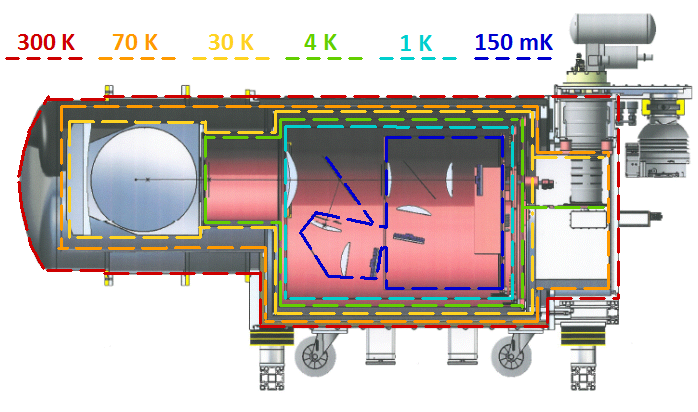
\includegraphics[width=.95\linewidth]{NIKA2_cryoStages.png}
      \caption{(Color online) Cross-section of the NIKA2 instrument illustrating the different cryogenics stages. The overall lenght of the instrument is around\,2.3 meters. The weight is close to 1300\,kg. The 150\,mK section includes the arrays, the dichroic, the polarizer and five HDPE lenses.}
         \label{Cryostat_cryo}
\end{figure}

The whole instrument includes thousands mechanical pieces, properly assembled for a total weight around 1.3\,tons. The weight of the 150\,mK stage is of the order of 80\,kg, including few kg of HDPE (High Density PolyEthilene) low-conductance lenses. Radiation screens are placed at 1\,K (still), 4\,K (pulses tubes second stage), 30\,K and 70\,K (pulses tubes first stages).

Selected inner parts, at each stage of temperature, are coated with a high emissivity mixture of black STYCAST 2850, SiC grains and carbon powder. This coating has demonstrated its effectiveness at millimeter wavelenghts in order to suppress unwanted reflections (\cite{Calvo2010}).

Magnetic screening is added on each cryogenics stage, employing high permittivity materials down to 1K, and a pure Aluminium superconducting screen at the 150\,mK and enclosing the detectors. The screening is mostly dedicated to: a) suppress the Earth magnetic field and its variations, in the instrument reference frame, during telescope slews in azimuth; b) suppress the magnetic field variations induced by the antenna moving in elevation. 

The operation of the cryostat does not require cryogenic liquids, and is fully remotely controlled. The whole cool-down procedure, largely automatised, lasts about five days. In particular, four days are required for the pre-cooling of the three coldest stages at around 4\,K. During the last 24 hours, the dilution procedure is started, allowing further cooling down to base temperature. Two additional days before stable observations are usually foreseen in order to ensure the perfect thermalisation of all the low-thermal-conductance optics elements like the lenses, filters and black coatings. The system is designed for long observational runs, and has showed so far the needed stability of the base temperature over roughly one month. The stability of the detectors temperature is better than 0.1\,mK over the duration of a typical observational block (scan), i.e. 15\,min.


 \subsection{The focal plane arrays}

Each array is fabricated on a single 4 inches High Resistivity (HR) Silicon wafer, on which a thin aluminium film (18\,nm) is deposited by e-gun evaporation under High Vacuum conditions. The use thin superconducting films has a double advantage: first of all, it increases the kinetic inductance of the material, making the detectors more responsive. And second, it maximises its normal state resistivity. An almost perfect match of the LEKID meander to the free space impedance of the incoming wave is thus allowed, ensuring a quantum efficiency exceeding 80\%. The NIKA2 pixels are all based on the Hilbert fractal geometry (\cite{Roesch2012}). 

In NIKA, we had adopted standard pixels coupled to a Coplanar waveguide (CPW) readout line, with bondings across the central line to suppress the spurious slotline modes, asociated to a break of symmetry between the ground planes at each side of the line itself. To optimize the optical coupling to the incoming milimetre radiation, we had adopted a back-illumination configuration, in which the light passes through the silicon wafer before reaching the pixels. To attenuate the refraction index mismatch, we had added a grid of perpendicular grooves on the bottom of the wafer, resulting an effective dielectric constant which is in between that of vacuum and that silicon (\cite{Goupy2016}). The total thickness of the silicon and the depth of the grooves were chosen to optimize the anti-reflection effect of the machined layer. A superconducting lid is then placed at an optimised distance after the detectors plane, acting as a $\lambda/4$ backshort. 

The same approach was originally planned for NIKA2. During the phase of the detectors development, however, we realised the practical limitations of the CPW coupling approach, in particular considering the thousands bondings required to ensure the exclusive propagation of the main mode. We then decided to study and test a different kind of transmission line, the microstrip (MS). This kind of feedline only supports one propagating mode, and is thus immune from the risk of spurious modes. Furthermore, the aluminium groundplane is located on the opposite side of the wafer with respect to the detectors, which might reduce the cross-coupling between different pixels.

This propagation mode shows an electric field oscillating, in the cold HR Silicon almost perfect dielectric, between the strip line (feedline) and the underlying ground plane (see figure  \ref{CPWvsMS}). The main drawback of the MS coupling lies in the fact that it forces, at least for dual-polarisation imaging applications, front-illuminating the detectors. It is thus more adapted for relatively narrow-band ($\Delta f / f  \leq 30 \%$) applications. This is however perfectly compatible with the NIKA2 goals.  

\begin{figure}[h]
   \centering
    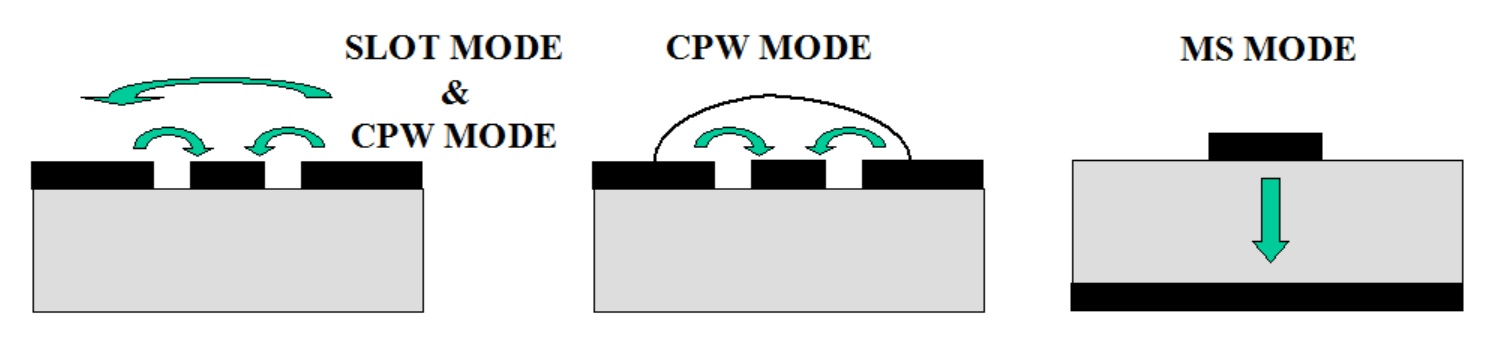
\includegraphics[width=.95\linewidth]{CPWvsMS.png}
      \caption{(Color online) In grey, the HR Silicon substrate, while in black the aluminium films is represented. Left: the CPW transmission line without across-the-line bondings, associated to strongly non-uniform performance of the detectors array. Center: the CPW, with bondings, configuration adopted in NIKA. Right: the microstrip (MS) configuration adopted in NIKA2, ensuring single-mode propagation and easiest implementation of very large arrays.}
         \label{CPWvsMS}
\end{figure}

In both cases, the distance between the pixels and the feedline is chosen in order to satisfy optimal coupling conditions. These are achieved when the coupling merit factor, $Q_c$, is of the same order as the internal merit factor $Q_i$ observed under typical loading condition. In the case of NIKA2, $Q_c\sim10,000$. A metal loop is added around each MS-coupled pixel to shield them from the feedline and achieve the wanted coupling without sacrificing the compactness of the pixels packaging (see figure \ref{Pixels}). 

In NIKA2, the 150\,GHz channel is equipped with an array of 616\,pixels, disposed to cover a circle with a 80\,mm diameter. Each pixel has a size of $2.8\times2.8\textrm{mm}^2$. This is the maximum size that can be adopted without degrading the telescope resolution, as it corresponds roughly to a $1 F \lambda$ sampling of the focal plane. The array is connected over four different readout lines, and shows resonance frequencies laying between 0.9 and 1.4\,GHz. The thickness of the Silicon substrate is around 150\,microns, calibrated to maximize the optical absorption at 150\,GHz. 

\begin{figure}[h]
   \centering
    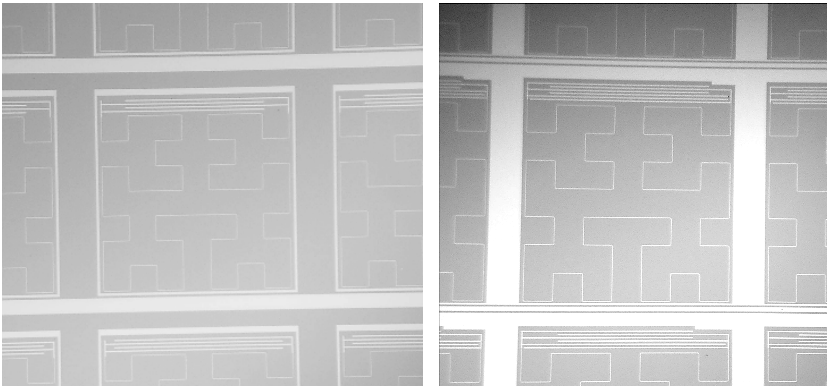
\includegraphics[width=.95\linewidth]{CPWeMS.png}
      \caption{(Color online) Left: a front-illuminated microstrip (MS) pixel for the 260\,GHz band of NIKA2. The pixels size is 2x2\,mm. Right: a back-illuminated coplanar waveguide (CPW) pixel used for the 150 GHz band in NIKA. The pixels size was in that case 2.3x2.3\,mm. Both designs are based on Hilbert-shape absorbers/inductors.}
         \label{Pixels}
\end{figure}

In the case of the 260\,GHz band detectors, the pixel size is $2\times 2\mathrm{mm}^2$, again to ensure a similar sampling of the focal plane. In order to fill the two 260\,GHz arrays, a total of 1140 pixels are needed in each of them. The smaller pixels dimensions compared to the 150\,GHz band lead to slightly higher resonance frequencies that are now comprised between 1.9 and 2.4\,GHz. Each of the 260\,GHz arrays is connected over eight different readout lines.  The thickness of the substrate is around 260\,microns, calibrated to maximize the optical absorption at 260\,GHz. 

\begin{figure}[h]
   \centering
    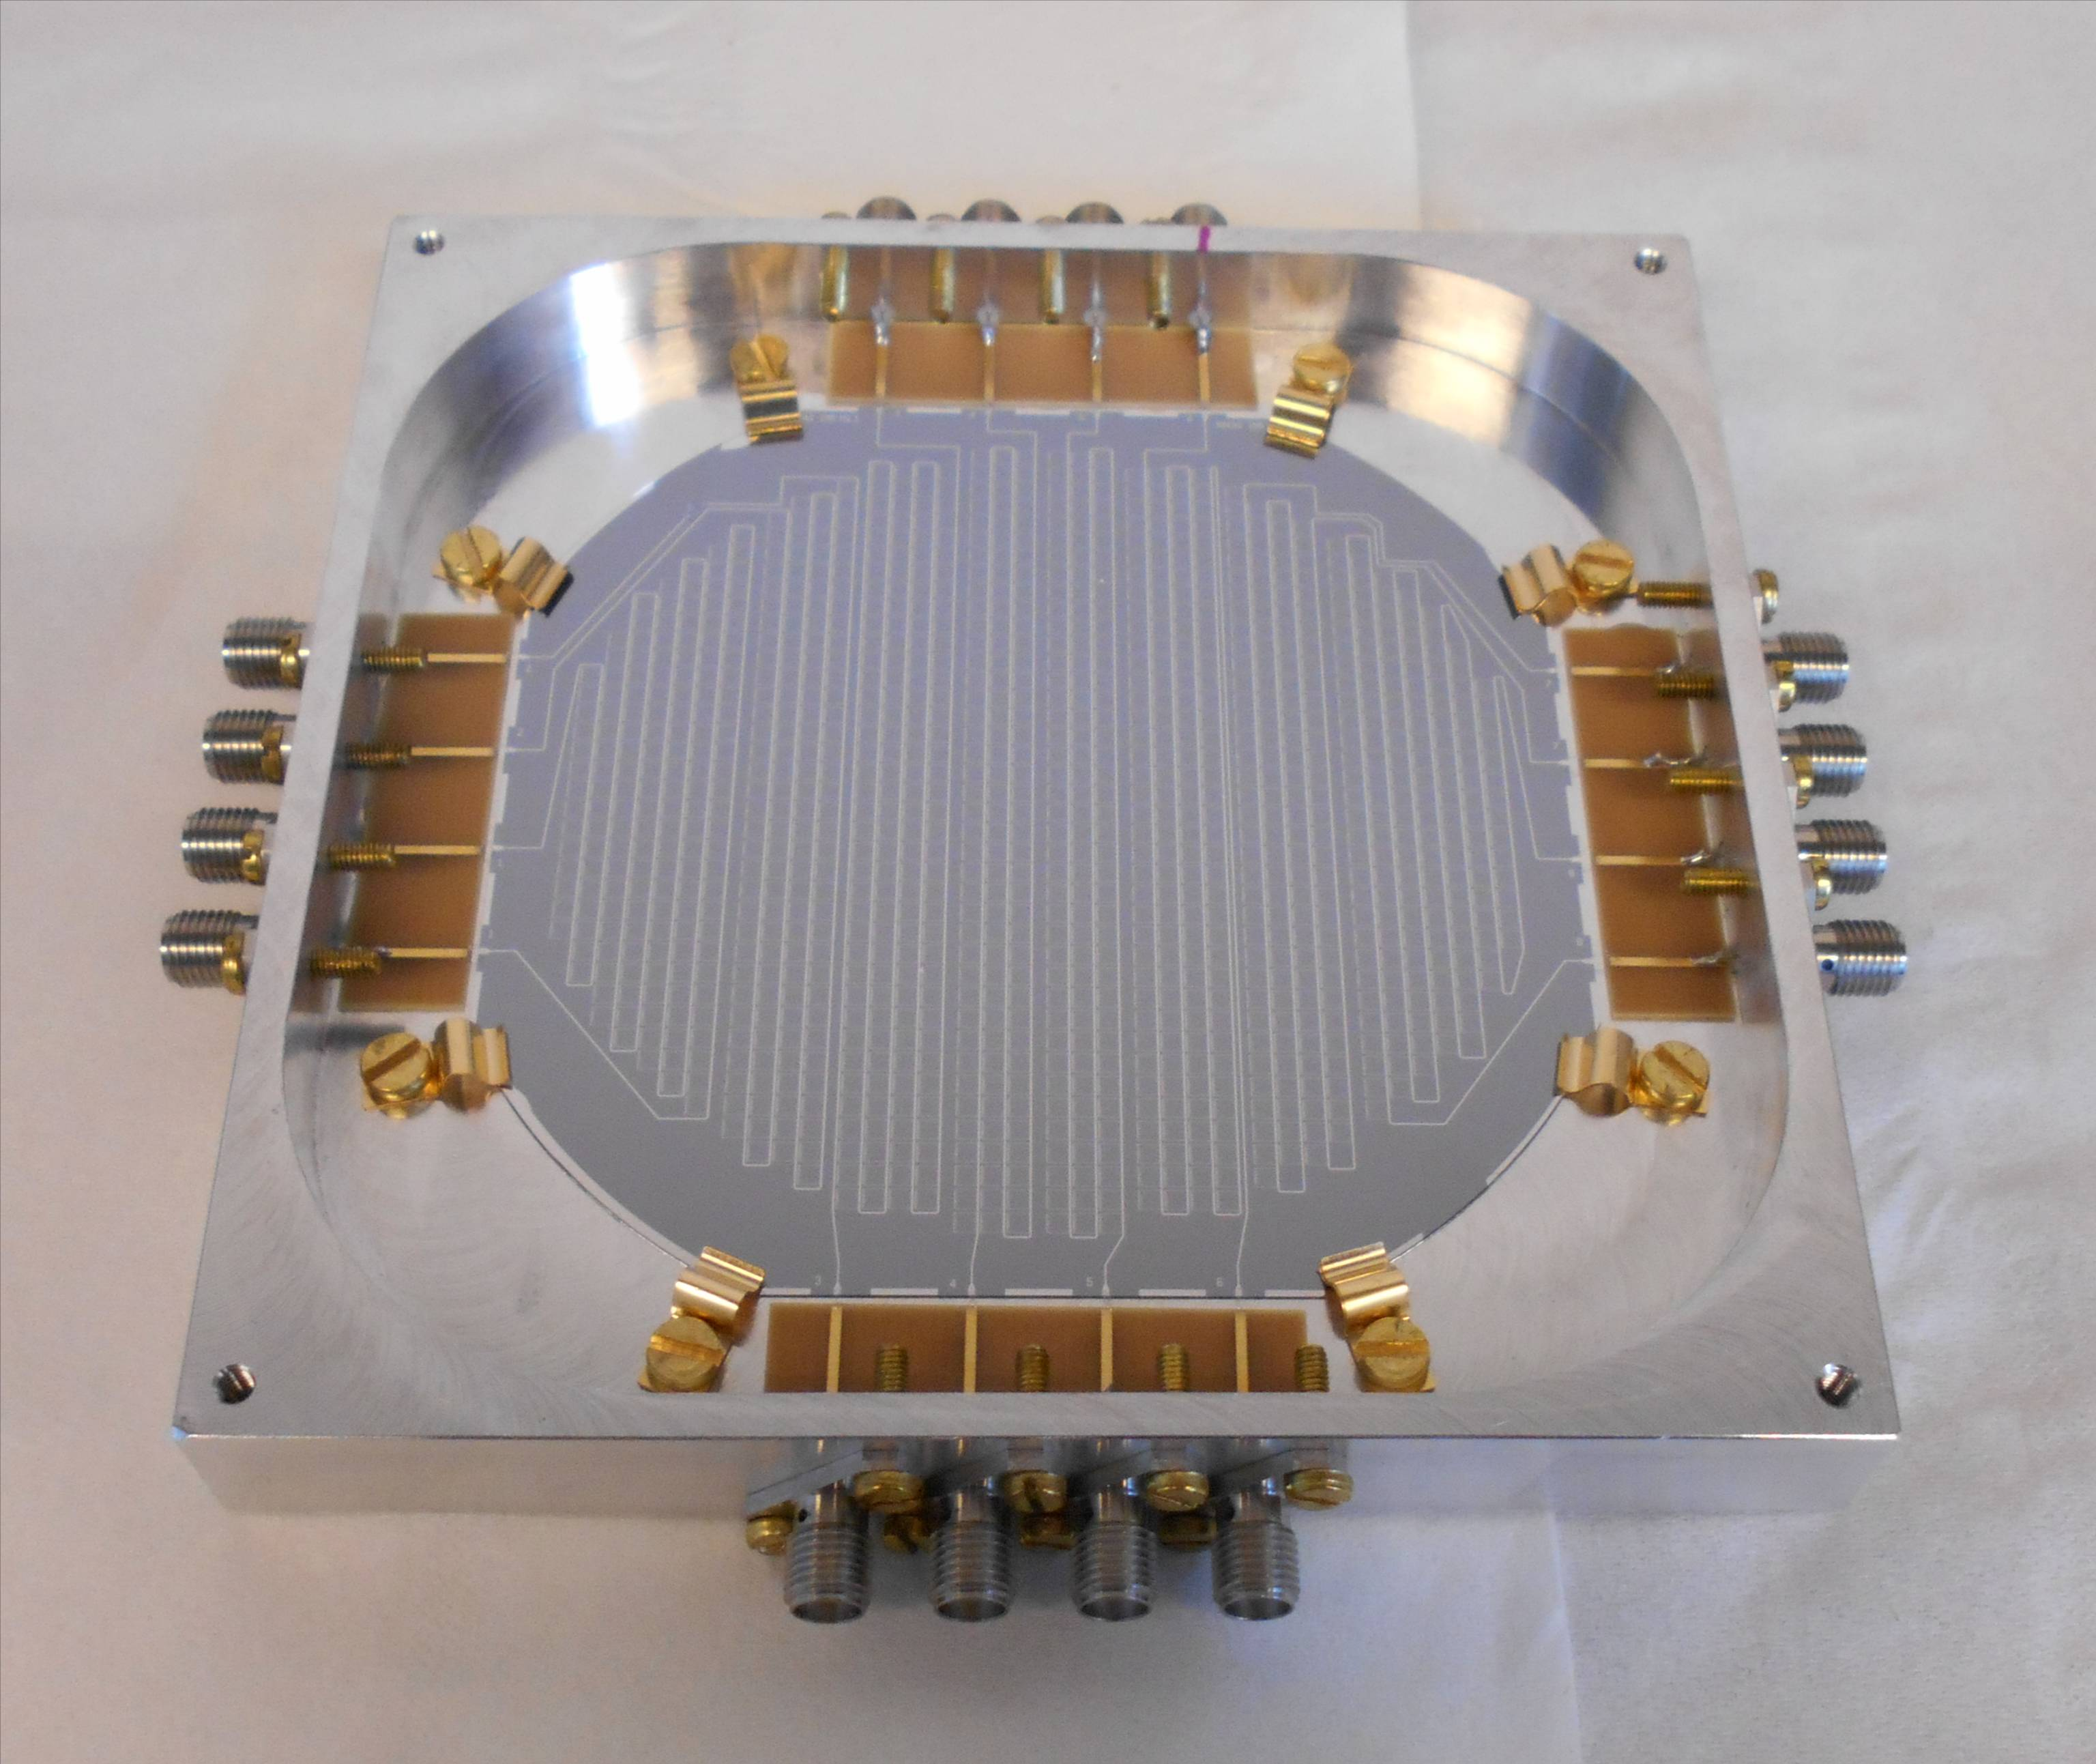
\includegraphics[width=.95\linewidth]{1mm_array.jpg}
      \caption{(Color online) One of the 260\,GHz NIKA2 arrays after packaging. The number of pixels designed for this array is 1140.}
         \label{Array}
\end{figure}

Please refer to figure \ref{Cryostat} for an illustration of the three arrays in the NIKA2 system.
 
\begin{figure}[h]
   \centering
   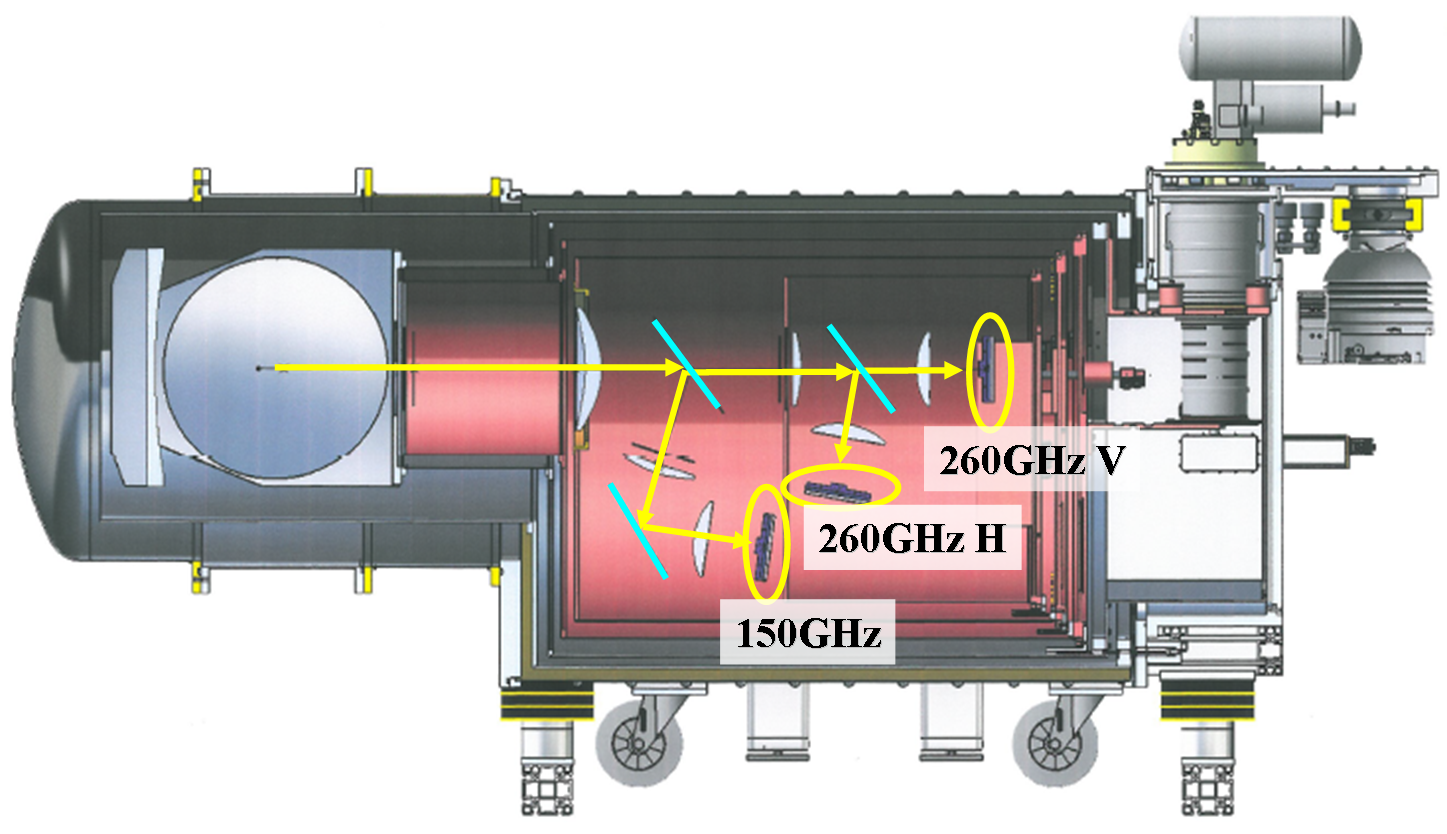
\includegraphics[width=.95\linewidth]{Fig1_cryo.png}
      \caption{(Color online) Cross-section of the NIKA2 instrument illustrating the three detectors arrays (150\,GHz, 260\,GHz-V and 260\,GHz-H). The optical axis and the photons direction of propagation is shown as well.}
         \label{Cryostat}
\end{figure}

Please refer to figure \ref{Cryostat} for an illustration of the three arrays in the NIKA2 system.

 \subsection{The cold optics}

In this section we describe in some detail the internal optics. More details concerning the telescope cabin optics are given in par.~\ref{Laboratory tests}.

NIKA2 is equipped with a reflective cold optics stage held at a temperature of around 30\,K. The two shaped mirrors (M7 and M8) are mounted in a specially-designed low-reflectance (\cite{Calvo2010}) optical box. The stray-light suppression is further enhanced by a multi-stage baffle at 4\,K.

The refractive part of the NIKA2 cold optics is mounted at 1 K and at the base temperature. The HDPE lenses, except those placed in front of the 260\,GHz arrays, are AR-coated. The coating is realised by a specific, custom machining of the surfaces. A 30-centimeters diameter air-gap dichroic splits the 150\,GHz (reflection) from the 260\,GHz (transmission) bands first. This dichroic, ensuring better flatness compared to the standard hot-pressed ones, has been developed in Cardiff specifically for NIKA2. A grid polarizer ensures then the separation of the two linear polarisations. Please refer to fig.~\ref{Cryostat} for a cross-section of the internal optics.

\begin{figure}[h]
   \centering
   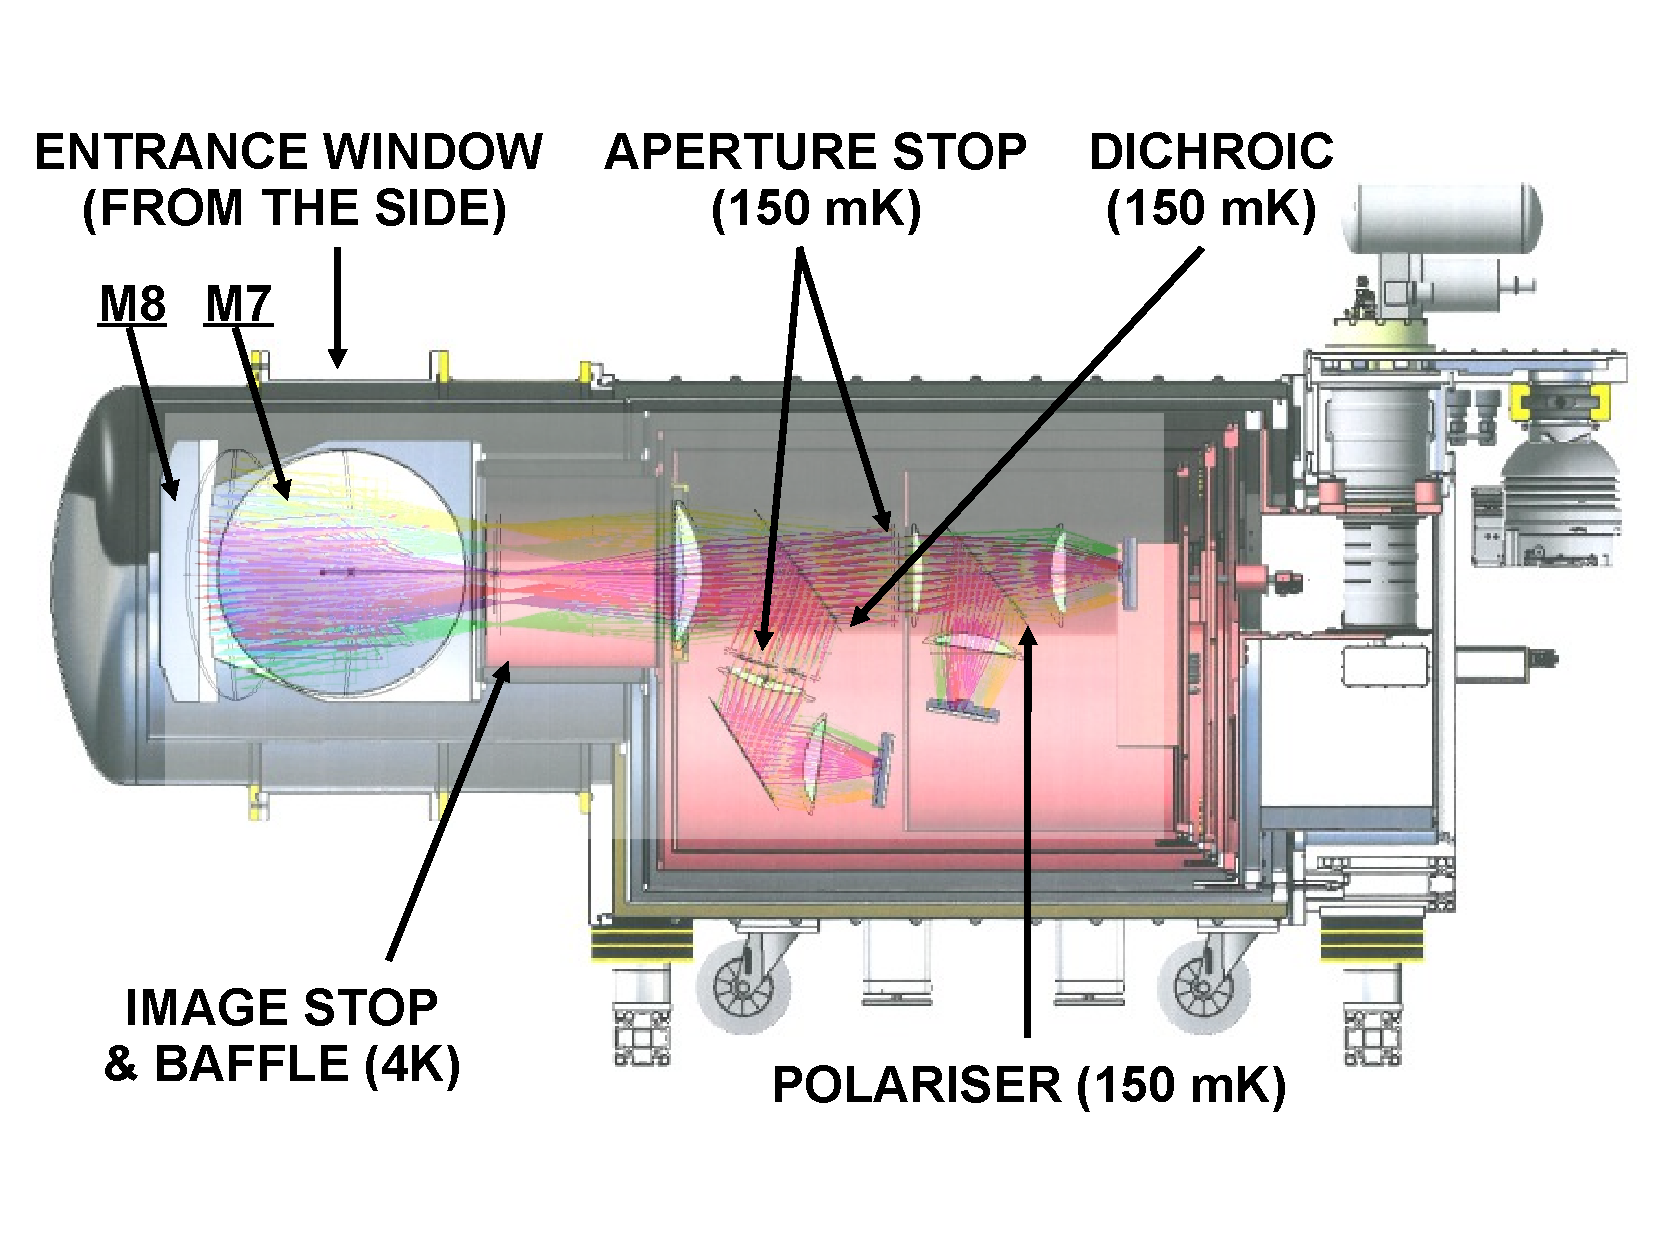
\includegraphics[width=.95\linewidth]{NIKA2_optics.pdf}
      \caption{(Color online) Cross-section of the NIKA2 instrument illustrating the cold optics and the main elements and surfaces described in the text.}
         \label{Cryostat_optics}
\end{figure}

The filtering of unwanted (off-band) radiation is provided by a suitable stack of multi-mesh filters placed at all temperature stages. In particular, three IR-cut filters are installed at 300\,K, 70\,K and 30\,K. Multi-mesh low-pass filters, with decreasing cutoff frequencies, are mounted at 30\,K, 4\,K, 1\,K and at base temperature. Band-defining filters, custom-designed and fabricated in Cardifi, are interposed at base temperature in order to optimally match the atmospheric windows. 

%POLARISATION FACILITIES (Andrea)
To exploit the NIKA2 polarisation capabilities, a modulator is added when operating the instrument in "polarized mode". It consists of a multi-mesh hot-pressed Half-Wave-Plate (HWP) (\cite{Pisano2016}) mounted in front of the cryostat window. The modulator uses a stepping motor and is operated at mechanical frequencies of up to 3\,Hz, corresponding to 12\,Hz concerning polarisation modulation speed. As already explained, and in order to detect the totality of the photons, the modulated polarised signal is then projected onto the two 260\,GHz arrays by the 45 deg. wire-grid polarizer at base temperature.  


 \subsection{The readout electronics}

One of the key advantages of the KID technology is the simplicity of the {\bf{cold electronics}} installed in the cryostat.
In NIKA2, each block of around 150 detectors is instrumented by a single coaxial line providing at one end the excitation and the readout at the other end. The excitation line, composed of stainless steel cables, are running from 300\,K down to sub-Kelvin temperature. They are properly thermalised at each cryostat stage, and a fixed attenuation of 20\,dB is applied at the 4\,K stage in order to suppress the 300\,K thermal noise. Each excitation line ends in an SMA connector (EXCitation input) and connected, through superconducting (Al) microbondings, to the silicon wafer holding the detectors. The approximate excitation power per pixel is usually of the order of 10\,pW.

On the readout side, the same types of microbondings are used to transfer the signal out of the focal plane and to make it available on a second SMA connector (MEASurement output). Then a superconducting (Nb) coaxial cable is used to connect directly the measurement output to the input of a low-noise cryogenics amplifier (LNA). The amplified signal provided by the LNA is transfered through the remaining cryostat stages (up to 300\,K) via stainless steel cables. 
The LNA, which operate at frequencies up to 2.5\,GHz, have noise temperatures comprised between 2\,K and 5\,K and are held at a physical temperature of about 8\,K.

The cryogenics amplifiers used by NIKA2 have been developed, fabricated and tested at the Yebes observatory and TTI Norte company, both located in Spain. The specifications of the amplifiers have been elaborated by the NIKA2 group.

NIKA2 is composed by a total of about 2,900 pixels and is equipped with 20 feed-lines. Thus, it employs 20 cryogenics amplifiers (four for the 150\,GHz array and eight each for the 260\,GHz arrays). The polarisation of these amplifiers is provided by a custom electronic box remotely controlled and allowing the optimizations of the individual biases according to the slightly different characteristics of the front-end high electrons mobility transistors (HEMT). 

\begin{figure}
\begin{center}
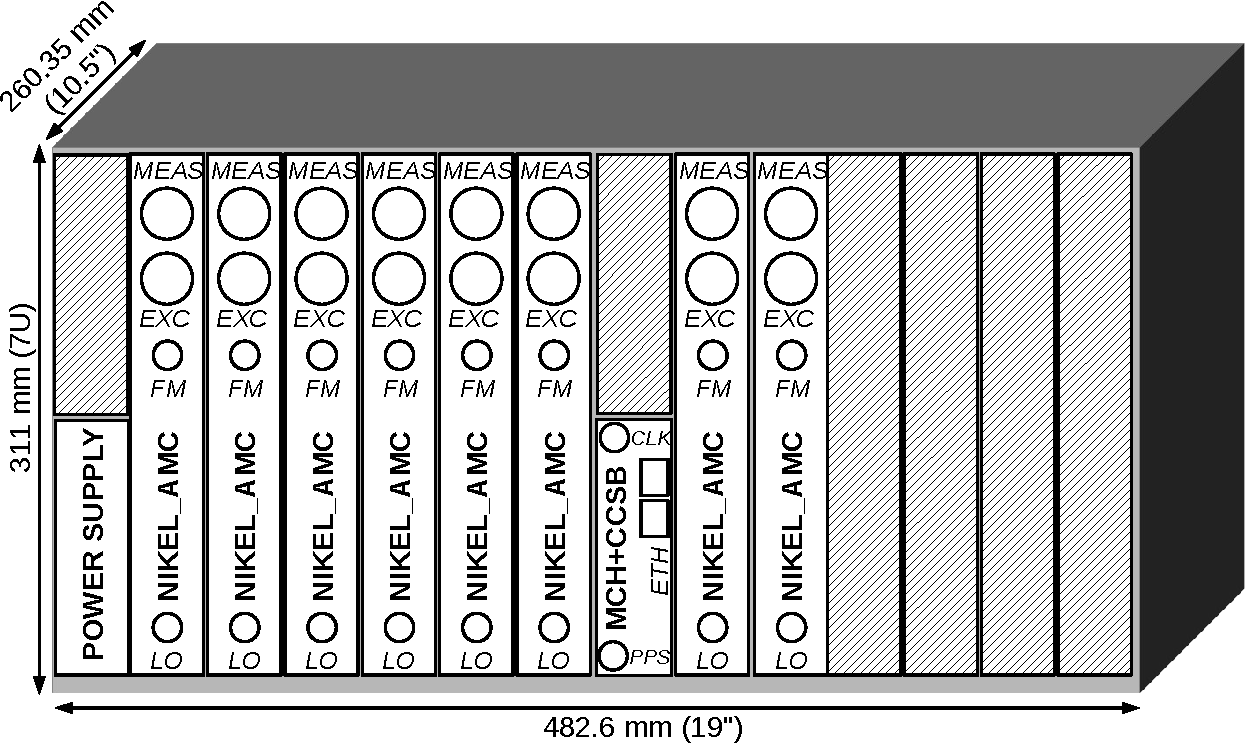
\includegraphics[angle=-90,width=0.45\textwidth]{NIKA_crate}
\caption{Overview of one array readout electronics crate.
It is equipped with 4 (or 8) readout boards lodged in Advanced Mezzanine Card slots (NIKEL\_AMC), one central and clocking and synchronization board (CCSB) mounted on the MicroTCA Carrier Hub (MCH) and one 600\,W power supply.
The crate allocated to the 150\,GHz channel uses 4 NIKEL\_AMC while the others use 8 NIKEL\_AMC boards.
\label{crateFig}}
\end{center}
\end{figure}

The \textbf{warm electronics} required to digitize and process the 2,900 pixels signals was specifically designed for that purpose.
It is composed of twenty readout cards (one by feed-line) named New Iram Kid ELectronic in Advanced Mezzanine Card format (NIKEL\_AMC).
As shown in fig.~\ref{crateFig}, the cards are distributed in three micro-Telecommunication Computing Architecture (MTCA) crates.
A central module, composed of a commercially available Mezzanine Control Hub (MCH) and of custom made mezzanine boards, is used to distribute a Rubidium reference clock (CLK) and a pulse per second (PPS) provided by GPS receiver and to control the crate.
This electronics is fully described in previous papers (\cite{Bourrion2012,Bourrion2016}).

In summary, the NIKEL\_AMC is composed of two parts: the radio-frequency (RF) part and the digitization and processing part.
The integrated RF part ensure the transition from and to the baseband part.
It uses the local oscillator (LO) input to perform up and down-conversions.
To instrument the 150\,GHz array (resonances from 0.9\,GHz to 1.4\,GHz) and the 260\,GHz arrays (resonances from 1.9\,GHz to 2.4\,GHz), the used LO input frequency are respectively 1.3\,GHz and 1.9\,GHz.
features a radio-frequency (RF).
The digitization and signal processing part, which is done at baseband, relies on channelized Digital Down Conversion (DDC) and their associated digital sine and cosine signal generators to build the excitation signal and to process the down-converted measurement signal.
The processing heavily relies on Field Programmable Gate Arrays (FPGA) while the interfacing to and from the analog domain is achieved by 1\,GSPS Analog to Digital and Digital to Analog Converters (ADC and DAC).
Finally, the electronics covers a bandwidth of 500\,MHz and can instrument up to 400\,KID in this bandwidth. In NIKA2 about 150 KID per board are instrumented, leaving a lot of room for placing dark excitation tones, and allow future developments of the instrument. 

It must be noted that for implementation reasons (\cite{Bourrion2012,Bourrion2016}) the excitation signal, nominally covering 500\,MHz is constructed by five DAC, each spanning 100\,MHz.



\subsection{Laboratory tests}
\label{Laboratory tests}

The NIKA2 arrays have been pre-characterised in laboratory under realistic illumination conditions. In order to compensate the absence of the telescope optics, we have added an additional lens at the cryostat input window. This lens is creating an image fo the focal planes onto our "sky simulator", described in previous papers (\cite{Catalano2014}, \cite{Monfardini2011}). A warm source, moved in front of the SS by means of an x-y stage, allows beams shape and arrays geometry (e.g. pixel-per-pixel pointing) characterisations. The sensitivity is calculated by excecuting calibrated temperature sweeps of the sky simulator, and measuring the signal-to-noise ratio of the detected signal. A photometric model has been elaborated, based on ray-tracing simulations and assuming reasonable overall optics (filters, lenses) transmission. In particular, the overall transmission of the instrument, mainly determined by the lenses and the filters, lies around 35\%. On top of that, the quantum efficiency of the detectors, integrated in the band of interest, is comprised between 60\% (260\,GHz arrays) and 80\% (150\,GHz array). The frequency sweep of the four lines making up to 150\,GHz array are shown in figure \label{VNA}. The average number of identified resonances over the twenty feedlines exceeds 90\% when compared to the number of pixels implemented by design. For example, in the case of the 150\,GHz array at least 580 beams are identified during laboratory tests, amounting more than 94\% of the total 616 implemented in the design. 

\begin{figure}[h]
\begin{center}
   \centering
    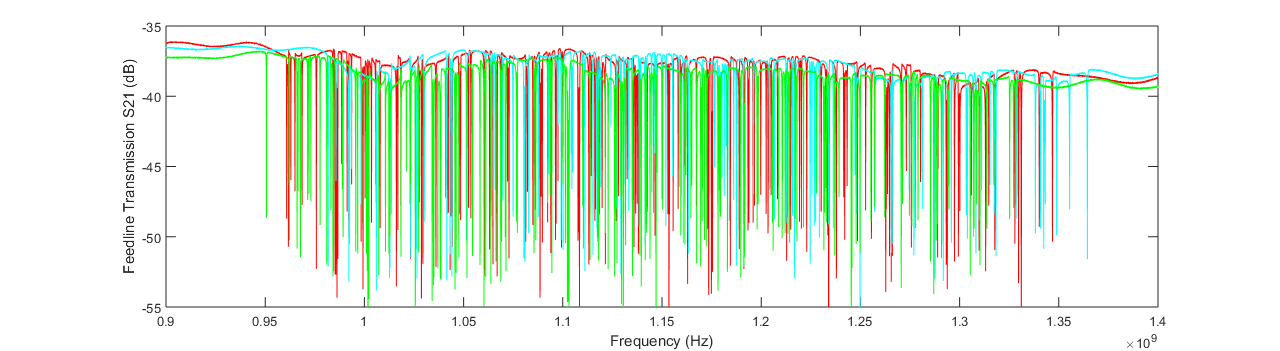
\includegraphics[width=1.05\linewidth]{VNA_scans_150GHz.png}
    \caption{(Color online) Resonances sweep for the four feedlines of the 150\,GHz array. The lines 1,2,3,4 are respectively shown in blue, red, cyan and green. The y-axis represents the transmission of the feedline (parameter S21) and is expressed in dB. Each dip correcponds to a resonance/pixel. About 94\% of the pixels are identified with a resonance and are sensitive to light.}
         \label{VNA}
\end{center}
\end{figure}

The measurable quantity, proportional to the incoming power per pixel, is the shift in frequency of each resonance (pixel) (\cite{Swenson2010}). That's why our noise spectral densities are expressed in Hz/Hz$^{0.5}$, and the responsivities are measured in Hz/K. Using the SS, we have estimated average responsivities of 1 and 2\,kHz/K at respectively 150 and 260 GHz. The average noise levels, for the two bands, are 1 and 3\,Hz/Hz$^{0.5}$, resulting in NET (Noise Equivalent Temperature) of the order of 1 and 1.5\,mK/Hz$^{0.5}$ per pixel at 150 and 260 GHz. These figures are calculated at a representative frequency of 5\,Hz. 

\begin{figure}[h]
\begin{center}
   \centering
    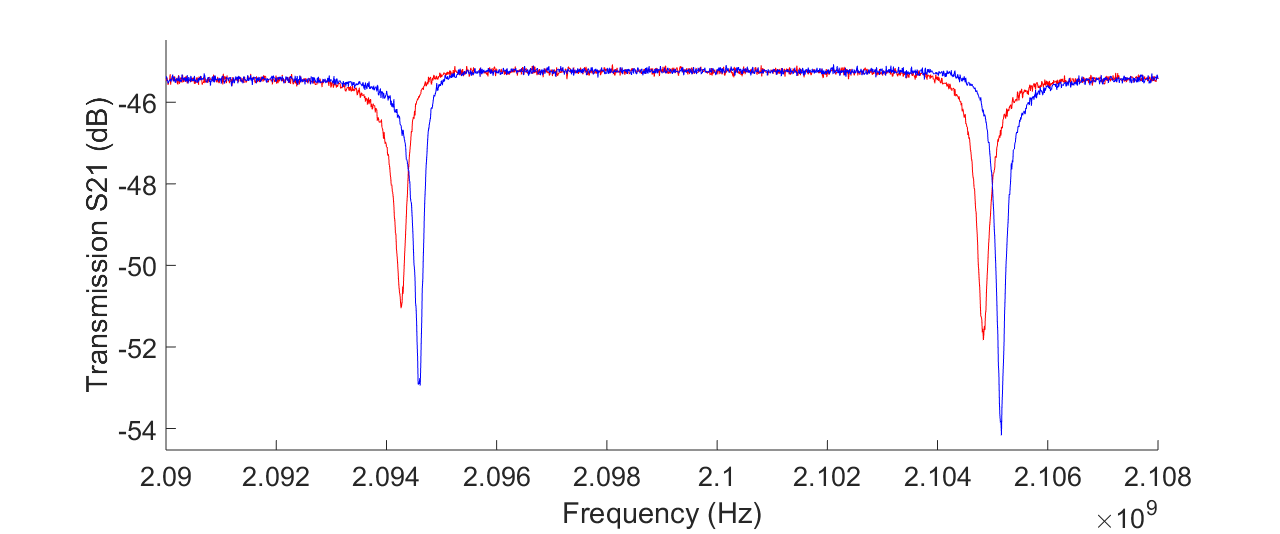
\includegraphics[width=1.05\linewidth]{Shift_f_260GHz.png}
    \caption{(Color online) Sky simulator testing (blue: the Sky Simulator is cold; red: 300K background) on two typical resonances of the 260\,GHz-V array. The measured average responsivity, i.e. the shift in frequency per unit temperature background variation, is around 2\,KHz for the 260\,GHz arrays and 1\,KHz/K in the case, not illustrated in figure, of the 150\,GHz.}
         \label{Shift_f}
\end{center}
\end{figure}

These figures are in line with the expectations. An example of Sky Simulator testing, allowing the measurement of the responsivity, is reported in figure \ref{Shift_f}. Noise spectra has been acquired as well in laboratory, with results then fully confirmed at the telescope, with NIKA2 observing the Sky. See the paragraph \ref{Noise and sensitivity} for a more detailed discussuin concerning the noise properties. 


The spectral characterisation of the arrays and the overall optical chain of NIKA2 has been achieved using a Martin-Puplett Interferometer (MpI) built in-house (\cite{Durand2008}) and specifically dedicated to instruments characterisation. The two arrays operating at 260\,GHz, mapping different polarisations, exhibit a slightly different spectral behaviour probably due to a tiny difference in the silicon wafer and/or Aluminium film thicknesses. The observed shift of the central frequency (265\,GHz for the V array versus 258\,GHz of the H) can be explained by about 5\,microns change in the substrate thickness.

\begin{figure}[h]
   \centering
%    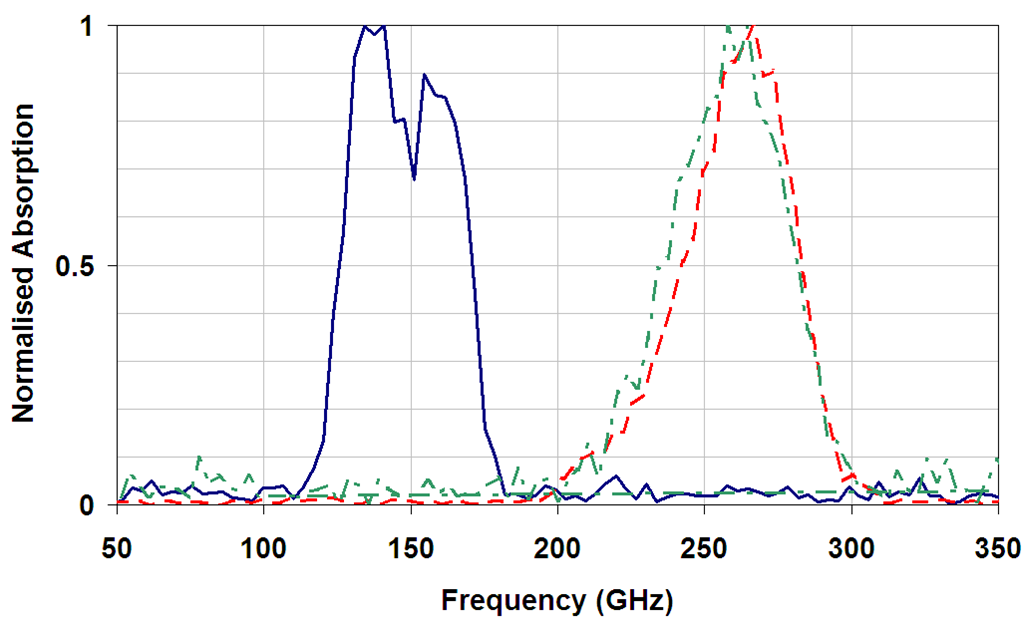
\includegraphics[width=0.9\linewidth]{Fig4_spectra.png}
    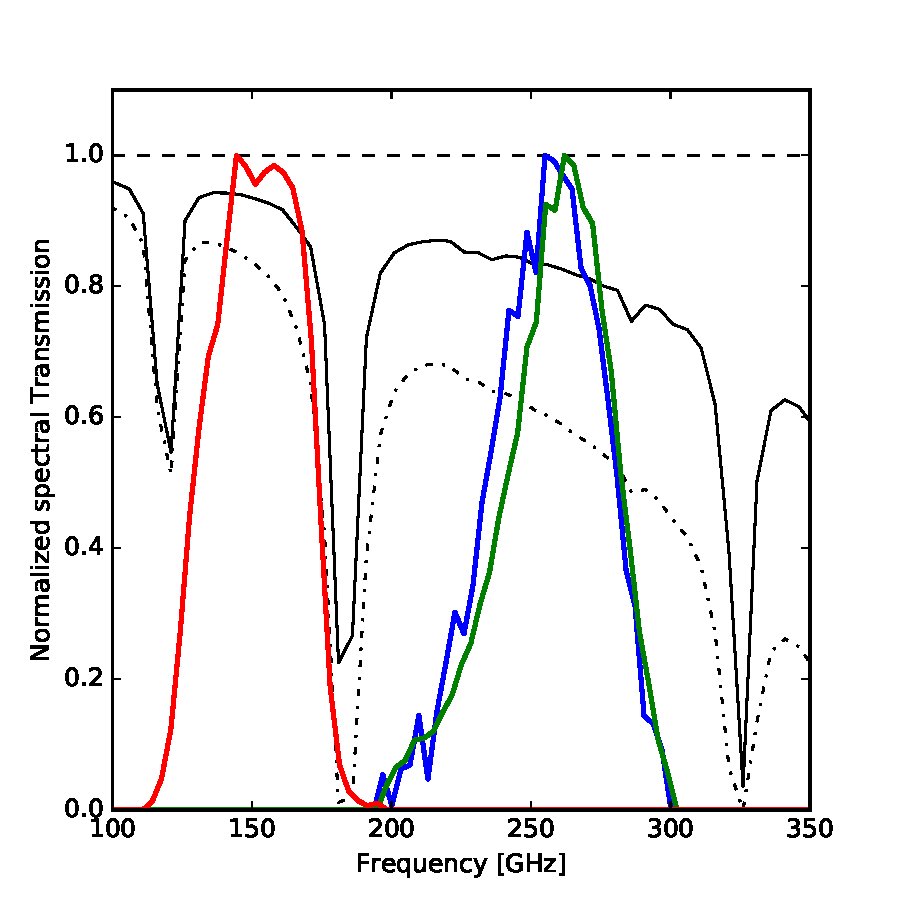
\includegraphics[width=0.9\linewidth]{atm_transmission.pdf}
      \caption{(Color online) NIKA2 spectral characerisation. Solid line (blue): 150 GHz array, FWHM: 126-170 GHz; dashed line (red): 260 GHz V, FWHM: 242-283 GHz; dashed-dotted line (green): 260 GHz V, FWHM: 235-281 GHz.}
         \label{Fig4}
\end{figure}

The Sky Simulator allows also a rough but important estimation of the stray-light, before installing the instrument at the telescope. By comparing measures acquired at several simulator distances compared to the cryostat window, we fit an equivalent 15\,K additional focal plane background due to the ambient temperature stray radiation. This is lower than the very best equivalent Sky temperature at Pico Veleta (20\,K), and confirms that NIKA2 is not limited by the stray-light. In comparison, in NIKA we had estimated around 35\,K additional background. 

In summary, the overall performance of the instrument, mesured preliminarily in laboratory, is in line with the NIKA2 specifications, paving the way for the installation at the telescope described briefly in the next paragraph. 

\subsection{The integration at the telescope}
\label{The integration at the telescope}

NIKA2 has been transported in pieces from the integration hall in Grenoble to the observatory on the end of September, 2015. Successful installation of the instrument took place in early October 2015 at the IRAM 30m telescope on Pico Veleta (Sierra Nevada, Spain). To prepare for this installation, the optics of the receiver cabin (M3, M4, M5 and M6) had been modified earlier in 2015 in order to allow increasing the telescope field-of-view up to the 6.5\,arc-min covered by NIKA2. M3 is the Nasmyth mirror attached to the telescope elevation axis. M4 is a flat mirror that can be turned manually in order to feed the beam either to NIKA2 or to the etherodyne spectroscopic instruments. The M5 and M6 non-flat mirrors are dedicated to the NIKA2 camera. 

\begin{figure}[h]
   \centering
    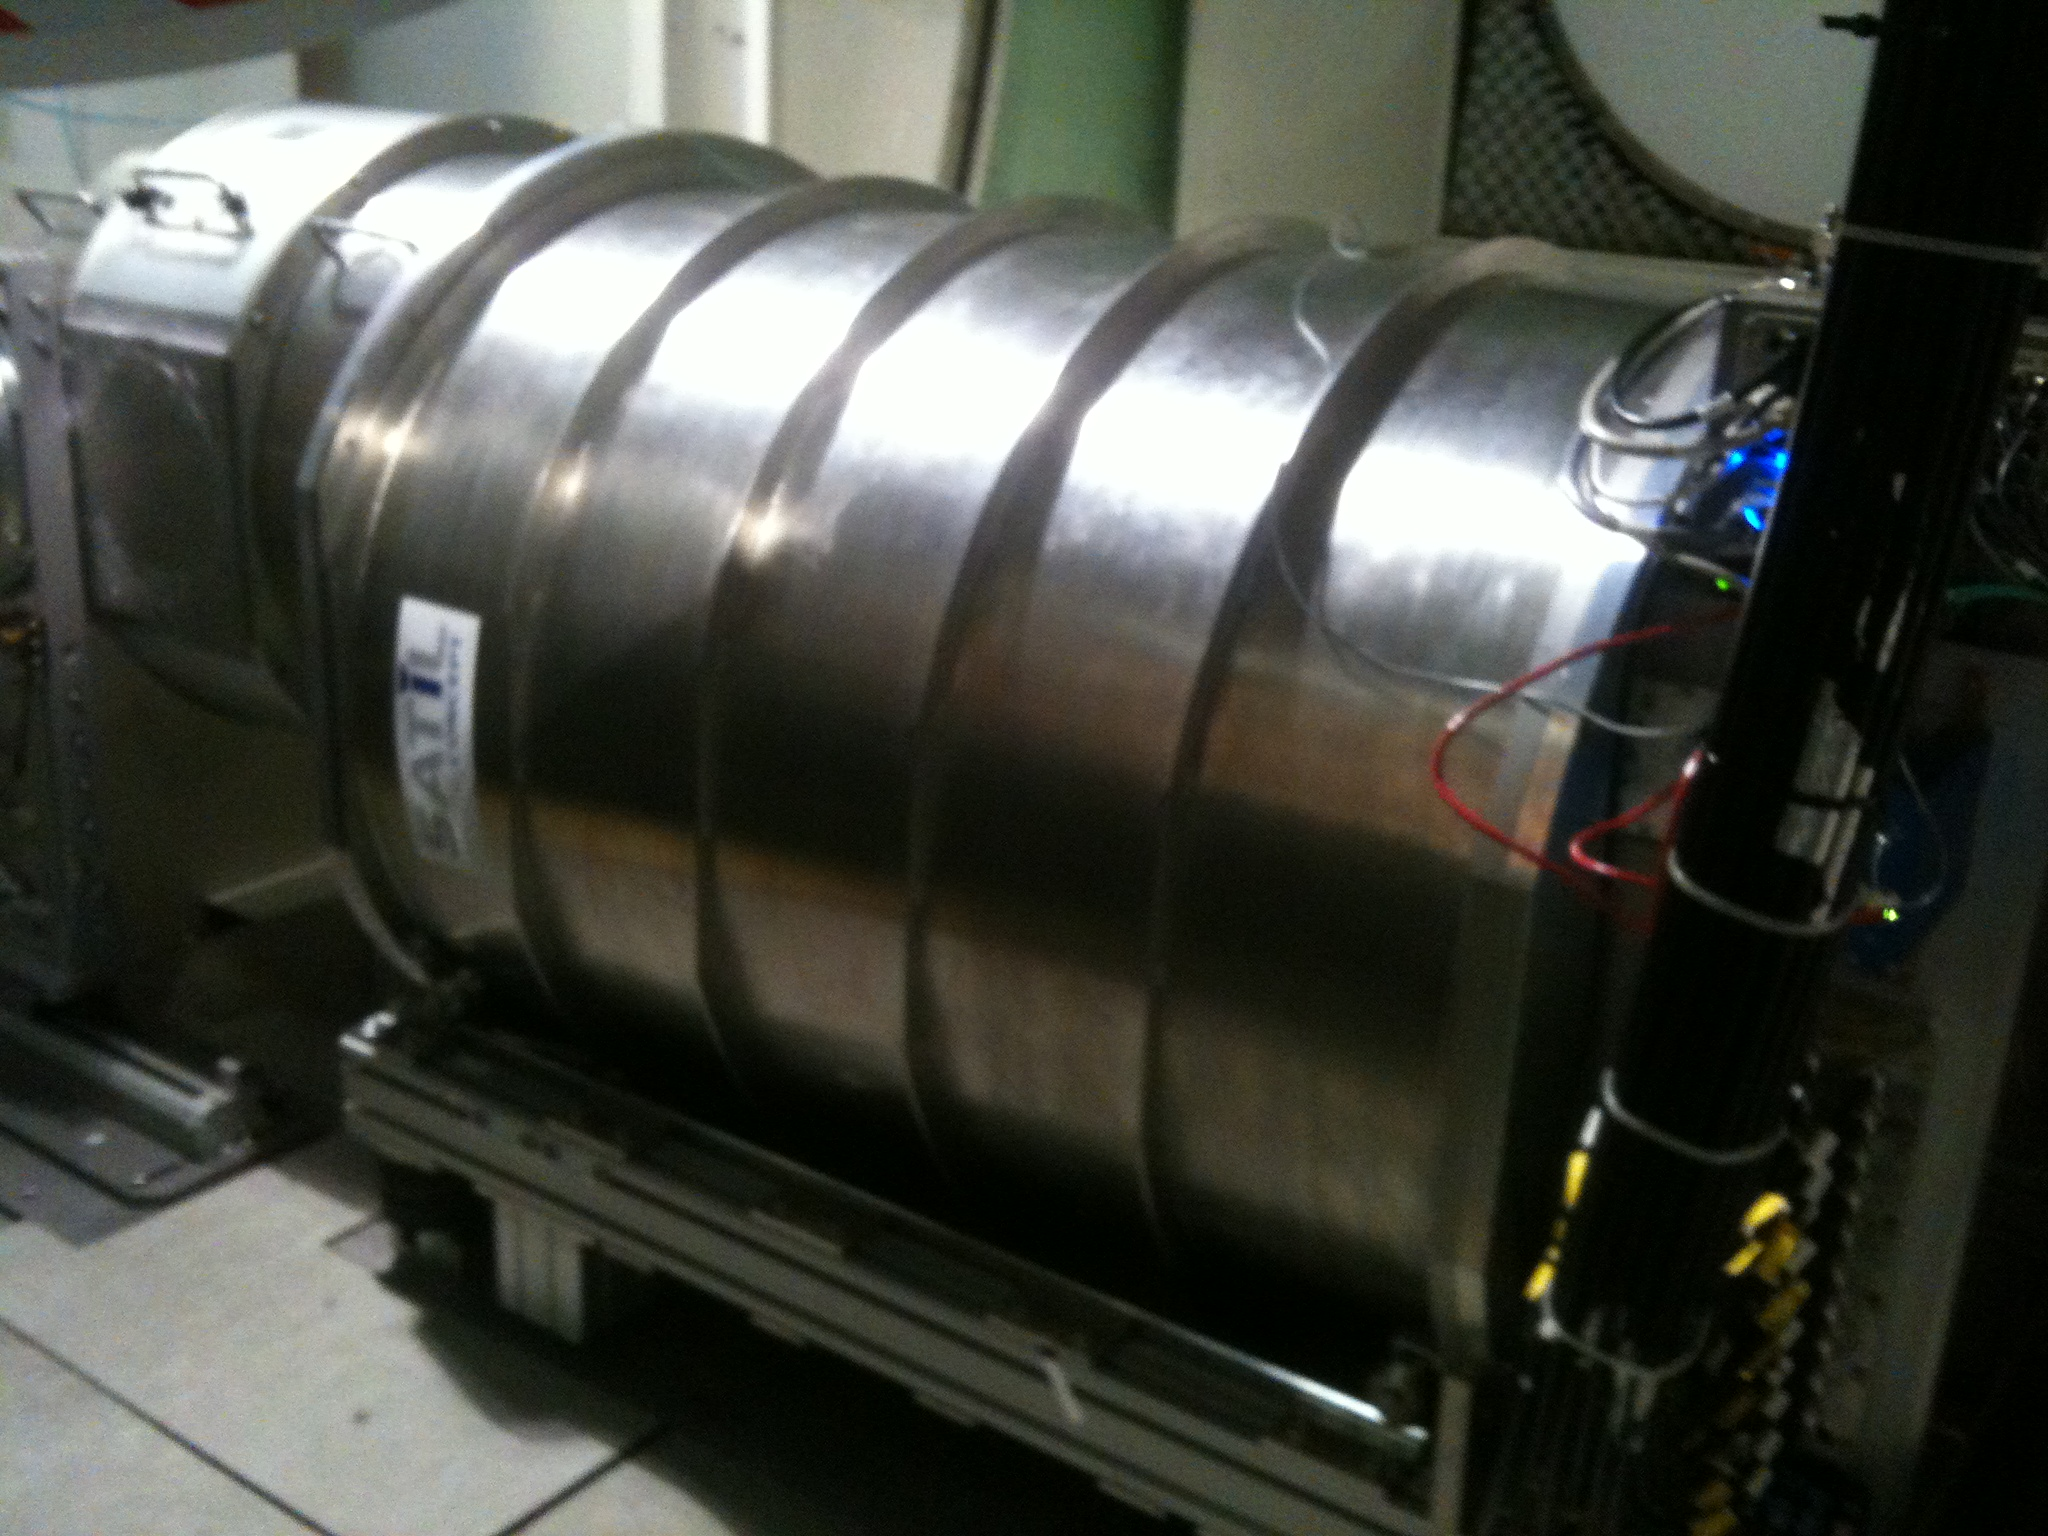
\includegraphics[width=.85\linewidth]{NIKA2cryo.jpg}
      \caption{(Color online) A picture of the NIKA2 cryostat installed in the 30-meters telescope receivers cabin end of September, 2015.}
         \label{Fig5}
\end{figure}

The whole installation, including the cabling of the instrument, was completed in around three days. The pulse-tubes pipes, 60-meters long, run through a derotator stage in order to connect the heads in the receiver cabin (rotating in azimuth) and the compressors located in the telescope basement (fixed). A single 1 Giga-bit ethernet cable ensured the communication of the NIKA2 instrument. The fourty radio-frequency connections (twenty excitation lines, twenty readouts) between the NIKEL\_AMC electronics and the cryostat, on the other side ot the receivers cabin, are realised using 10-meters long coaxial cables. 

The optical alignment between the instrument and the cabin optica has been achieved using two red lasers. The first was set shooting from the center of the NIKA2 input window, through the telescope optics and reaching the vertex. The second laser is mounted on the telescope elevation axis, reaching then, through the M4, M5 and M6 mirrors, the NIKA2 window. In both cases, we have adjusted the cryostat position and tilt to achieve good alignment. Once the best laser alignment is found, NIKA2 is equipped with an automatic system of pneumatic actuators and position detectors able to adjust the cryostat height and tilt and keep it stable. 

The first cryostat cooldown started immediately afterwards, and was achieved on October, 7th, 2015 after the nominal four days dedicated pre-cooling and less than 24 hours during which the helium isotopes mixture is condensed in the so-called "mixing chamber" and the dilution process is started. 

The first technical tests demonstrated immediately that all the detectors were functional and exhibited responsivity and noise in line with the laboratory measurements presented in the previous paragraph. The first commissioning run could then start.


%______________________________________________________________



\section{The calibration procedures}

The photometry is reconstructed down to the required few percent level thanks to three distinct procedures applied by default. First, we have implemented an electrical calibration acting directly on the KID and specific to NIKA and NIKA2 (par.~\ref{Internal detectors calibration}). Secondly, we measure, as any other instrument, a flat-field using known sources (par.~\ref{On-sky calibration}). Lastly, the atmosphere opacity correction is calculated in real time thanks to the large dynamics and linearity of the detectors (par.~\ref{Atmospheric attenuation correction}).

\subsection{Internal detectors calibration}
\label{Internal detectors calibration}
When radiation is absorbed in a KID, it breaks part of the superconducting carriers (Cooper Pairs) and creates an excess of unbound electrons (quasi-particles). This changes the impedance of the film and shifts the resonance frequency $f_0$ of the illuminated KID to lower values.
%[For small variations of the absorbed power, delta f_0 is directly proportional to $\delta P$.] 
The standard way to readout a pixel is to excite it with a tone at $f_0$ and to monitor how the In-phase ($I$) and in-Quadrature ($Q$) components of the transmitted signal are modified by the changes in $f_0$. For NIKA2 we adopted a different strategy, already developed for NIKA. Instead of using an excitation at a fixed frequency, we rapidly modulate between two different readout tones, $f^+$ and $f^-$, just above and just below $f_0$. The tones are separated by $df=f^+-f^-$. This modulation technique allows to measure, for every acquired data sample, both the values of $I$ and $Q$ and the variation $dI$, $dQ$ that is induced by the chosen frequency shift $df$. When the optical power on the detectors changes by an amount $\Delta P_{opt}$, a variation $\Delta I$, $\Delta Q$ is observed between successive data samples. The $dI$, $dQ$ values can then be used as a calibration factor to associate to the observed $\Delta I$, $\Delta Q$ the corresponding change in the resonance frequency $\Delta f_0$, and thus measure $\Delta P_{opt}$. More details on the modulated readout technique can be found in \cite{Calvo2013} and \cite{Catalano2014}.

The advantage of this solution is that the $dI$, $dQ$ values are evaluated for every data sample. If the load on the detectors change (e.g. due to variations in the atmospheric opacity), the exact shape of the resonance feature of each pixel will change, but since the calibration factor $dI$, $dQ$ is updated in real time it will take this effect into account. Its use thus strongly increases the photometric accuracy of the instrument.

Furthermore, knowing both the $I$, $Q$ and the $dI$, $dQ$ values we can also estimate the current position of a KID resonance with respect to the position of the corresponding excitation tone. In the ideal situation, these two positions should coincide. In reality, changes in the background load can make the resonances drift by a large amount. Thanks to the modulated readout, when this happens the excitation tones can be rapidly re-tuned to keep track of the new resonance positions. This tuning procedure allows us to always readout the KID with optimally placed tones, which prevent any degradation in the sensitivity of the detectors.


\subsection{Atmospheric attenuation correction}
\label{Atmospheric attenuation correction}

The sky maps are corrected for the atmospheric contribution rescaling the observed signal by what that would be obtained in the absence of atmosphere. The corrected brightness is:

\begin{equation}
S^{Star} =  S^{Ground} \cdot e^{ x \tau_{scan}}.
\end{equation}

Where $\tau_{scan}$ is the opacity of the atmosphere and $x$ corresponds to the airmass at the elevation of the considered map\footnote{The airmass is the volume of air defined by its temperature and water vapor content. By assuming a homogeneous plane-parallel atmosphere, the relation between the airmass and the elevation of the telescope becomes $x = sec(\delta)$, where $\delta$ is the average elevation.}.
In NIKA2, the opacity is measured via the elevation scan technique (skydip). This procedure was successfully tested in the NIKA pathfinder producing a low-level dispersion of the derived opacity at different elevations. The details of this technique and its agreement with the Atmospheric Transmission at Microwaves (ATM) model \cite{2001IEEE....49.1683C} are described in \cite{Catalano2014}. Briefly, the underlying idea is to replace the opacity delivered by the resident IRAM tau-meter that performs elevation scans continuously at a fixed azimuth at 225~GHz, with a direct measurement that uses the NIKA2 instrument itself as a tau-meter. Using this procedure we can directly derive an opacity integrated in the NIKA2 bandpasses and at the same position of the source in the considered map. 
During a skydip, the telescope performs ten elevation steps from 19 to 65 degrees. For each step we acquire about twenty seconds of useful signal. The relation between the resonance frequency of each pixel and the airmass is given by the following equation:

\begin{equation}\label{eq:skydip}
S^{Ground}_{skydip} = C_0 + C_1 T_{atm}[1 - e^{- x \tau_{skydip}}].
\end{equation}

Where $F^{Ground}_{skydip}$ is the acquired signal which corresponds to the
absolute value of the shift in the resonance frequency for each pixel, $C_0$ is the
instrumental offset corresponding to the resonance frequency for the
considered pixel at zero opacity, $C_1$ is the calibration conversion factor in
$\mathrm{Hz/K}$, $T_{atm}$ is the equivalent temperature of the
atmosphere, $\tau_{skydip}$ is the sky opacity during the skydip, and $x$ is the airmass.

A skydip shows that the value of $tau$ is common between pixels of the same channel as expected. Coefficients  $C_0$, $C_1$ depend on the response of the detectors. Since the non-linearities of the KID frequency signal are negligible in the considered range of backgrounds, the coefficients can be applied to all the observing campaign to recover the opacity of the considered scan. This is
obtained by inverting Eq \ref{eq:skydip} on the considered map. In Fig.~??? we present the evolution of the opacities for several map of the NIKA2 commissioning  in February-March 2016 compared to the IRAM tau-meter.

%______________________________________________________________

\section{Observations and performance}

The first astronomical light has been achieved on the 7th October 2015. A first technical run followed immediately. Two more commissioning runs, for a total of about three weeks on Sky, have been carried out in November, 2015 and January, 2016. In this paragraph we summarize the main results obtained.

\subsection{Focal plane reconstruction}

\begin{figure*}[h]
   \centering
%    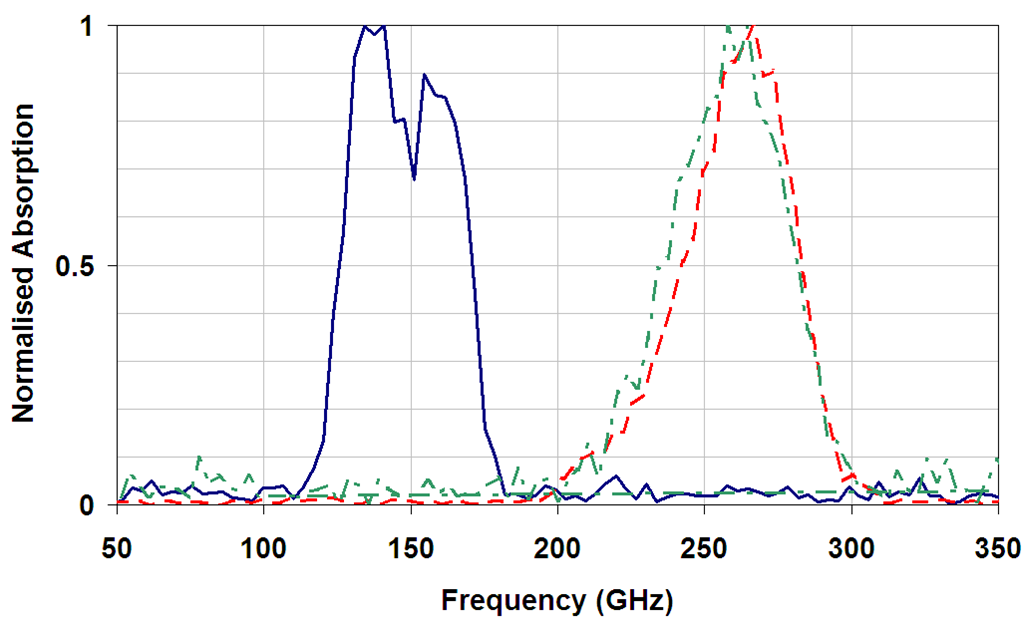
\includegraphics[width=0.9\linewidth]{Fig4_spectra.png}
    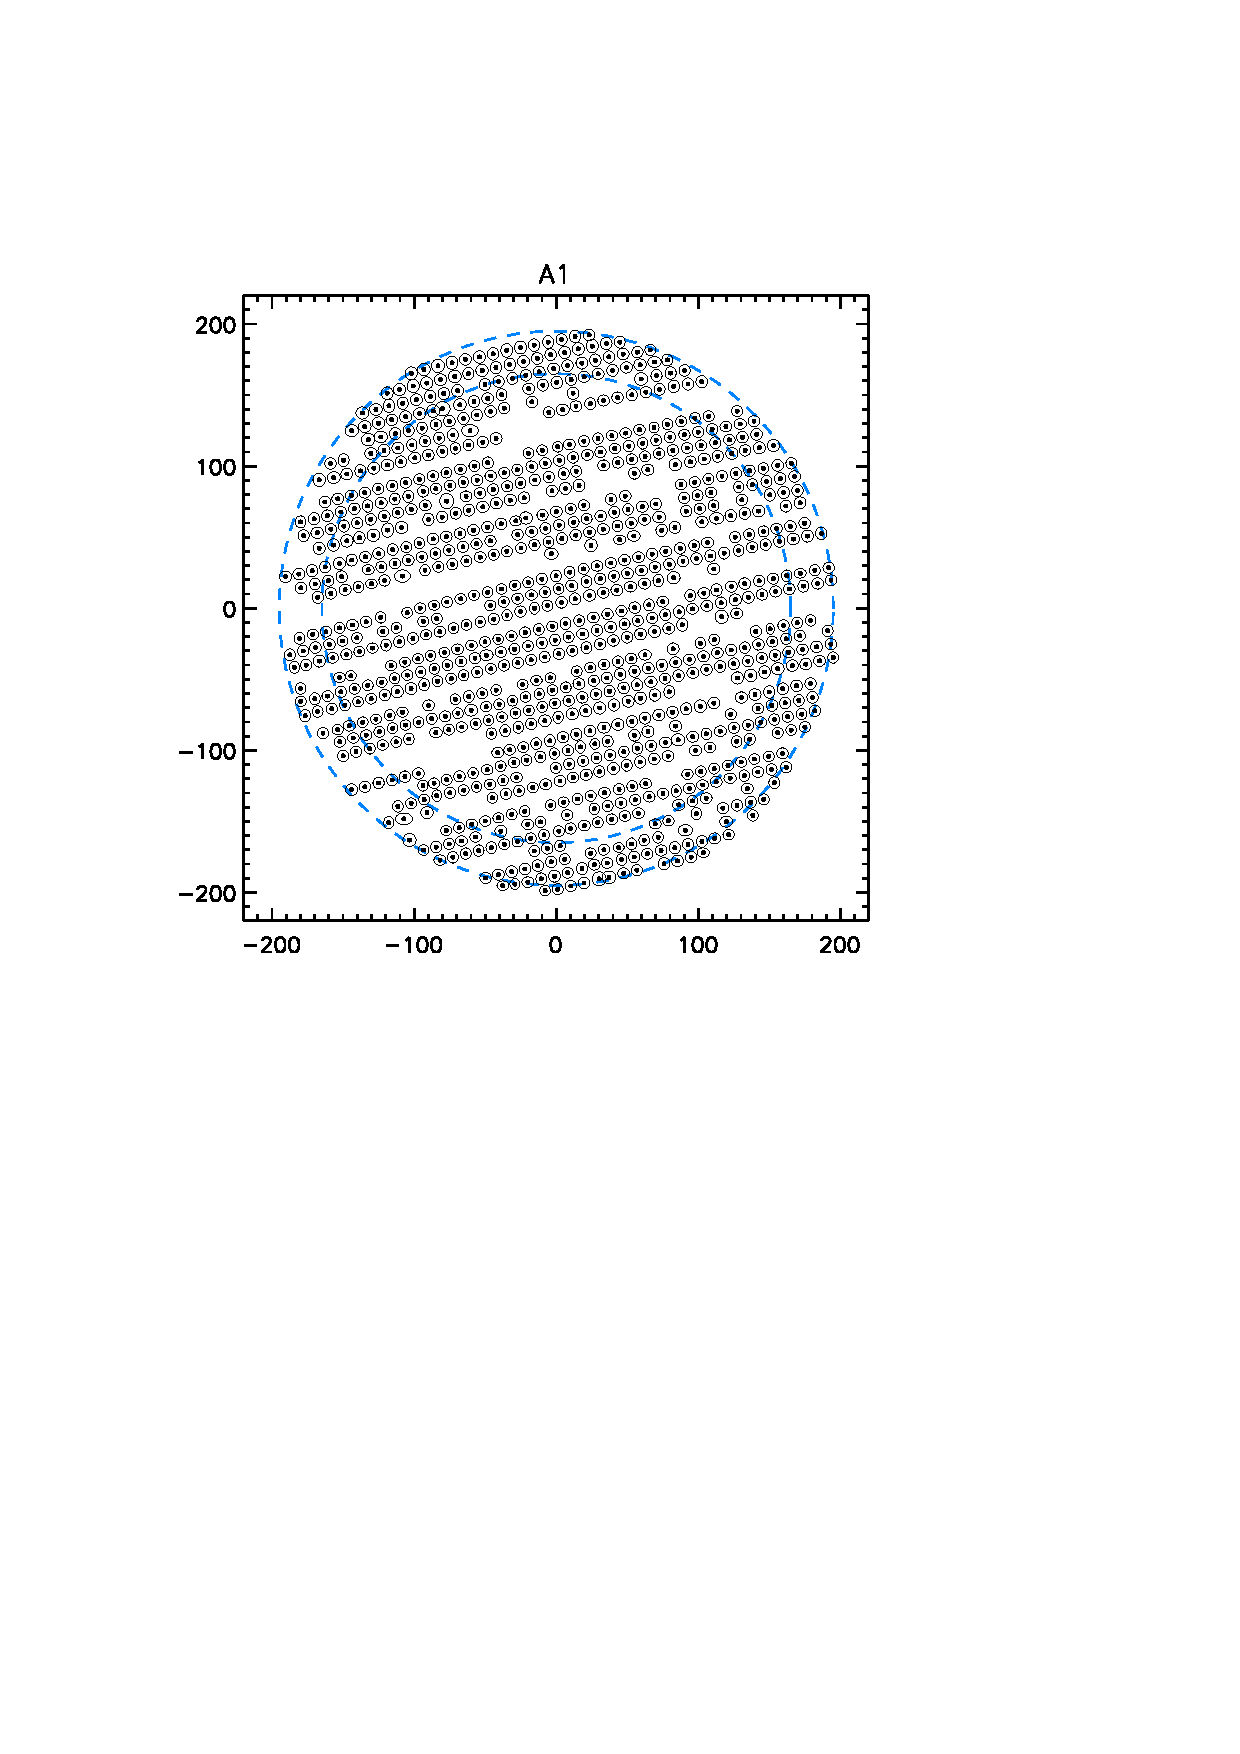
\includegraphics[trim=2cm 14cm 5cm 4cm, clip=true,width=0.33\linewidth]{A1_fwhm_valid.pdf}
   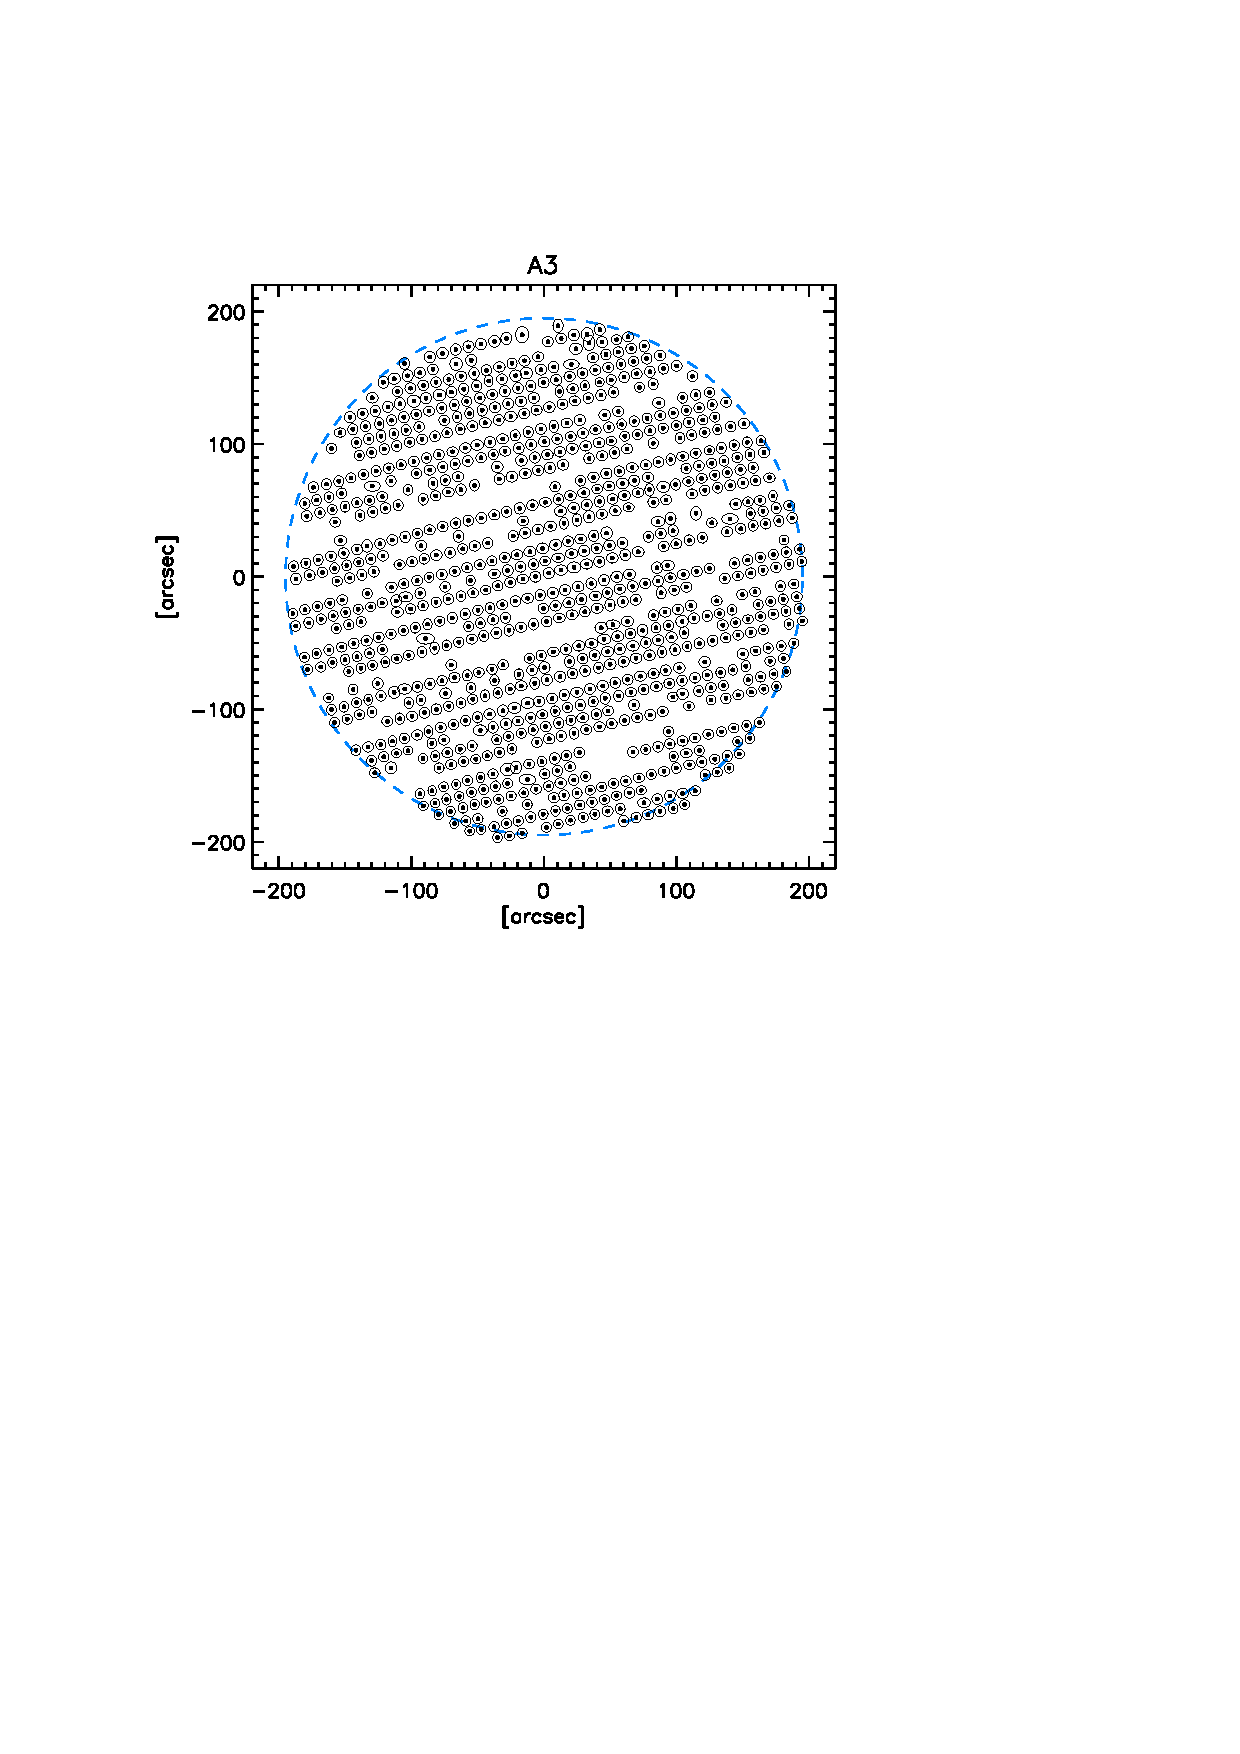
\includegraphics[trim=2cm 14cm 5cm 4cm, clip=true,width=0.33\linewidth]{A3_fwhm_valid.pdf}
   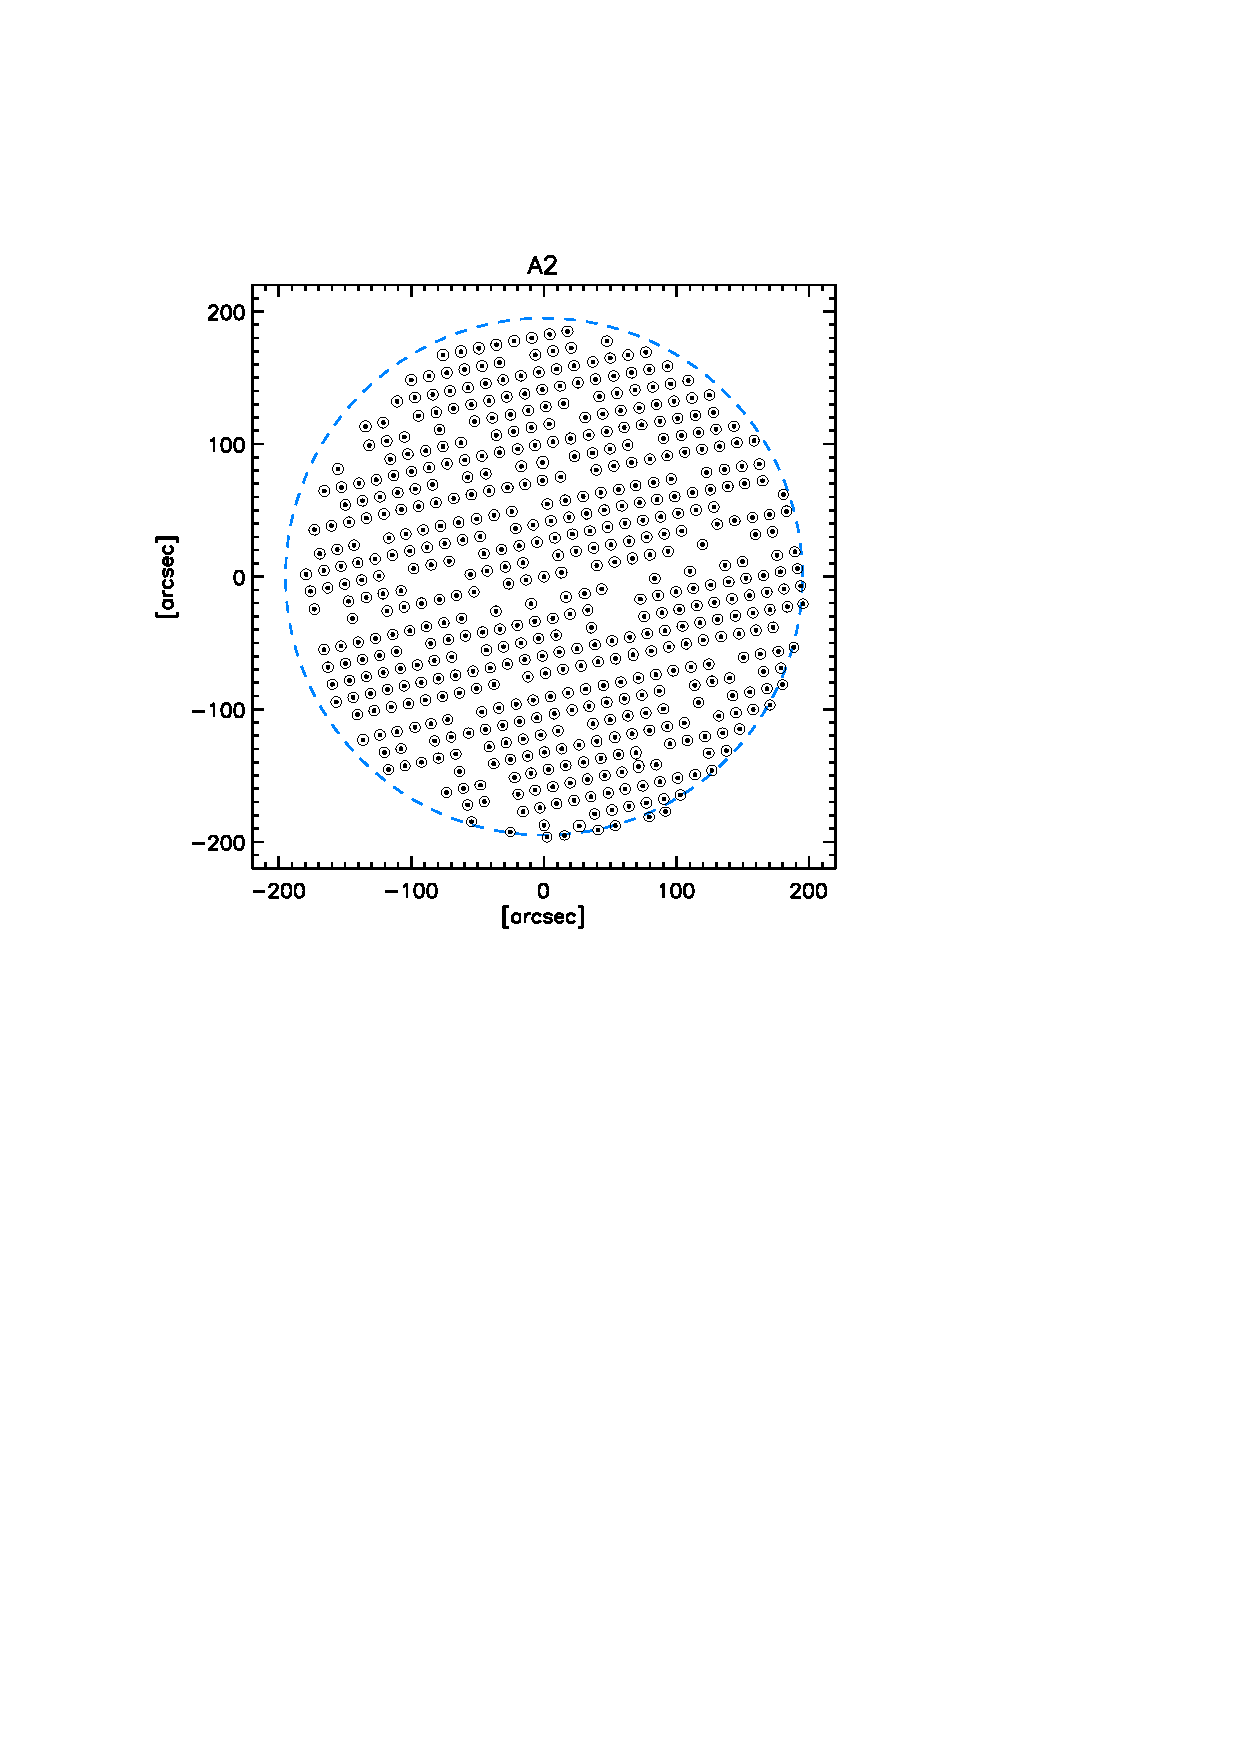
\includegraphics[trim=2cm 14cm 5cm 4cm, clip=true,width=0.33\linewidth]{A2_fwhm_valid.pdf}
       
      \caption{From left to right, detectors positions for arrays A1, A3, and A2. The three plots show the detectors that have seen the sky and passed the quality criteria for at least two focal plane reconstructions during Run10 (901, 903, 533 for A1, A3 and A2, respectively).}
         \label{fig:focalplane}
\end{figure*}

Figure~\ref{fig:focalplane} shows the position of the array A1, A3 and A2 detectors in the NIKA2 FOV. For each detector the ellipse symbol size and ellipticity
are proportional to the main beam FWHM and the ellipticity of the full beam assuming a 2D Gaussian. 

\begin{figure*}[h]
  \centering
  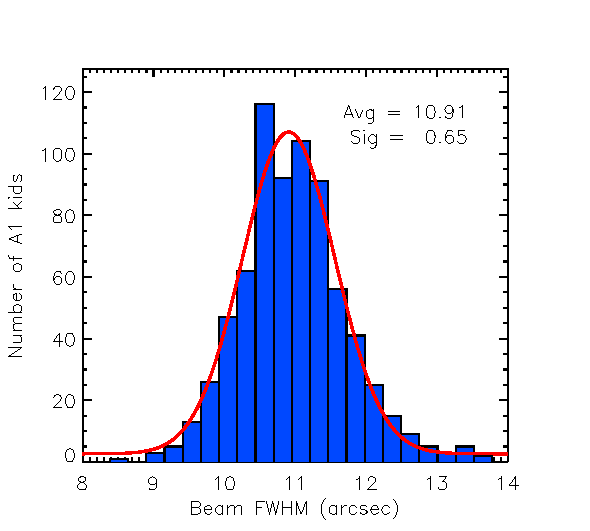
\includegraphics[clip=true,width=0.33\linewidth]{plot_histo_A1_fwhm_20170424s123.pdf}
  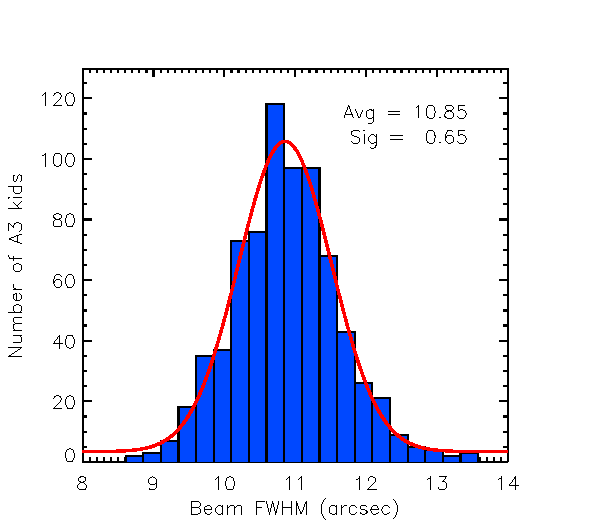
\includegraphics[clip=true,width=0.33\linewidth]{plot_histo_A3_fwhm_20170424s123.pdf}
  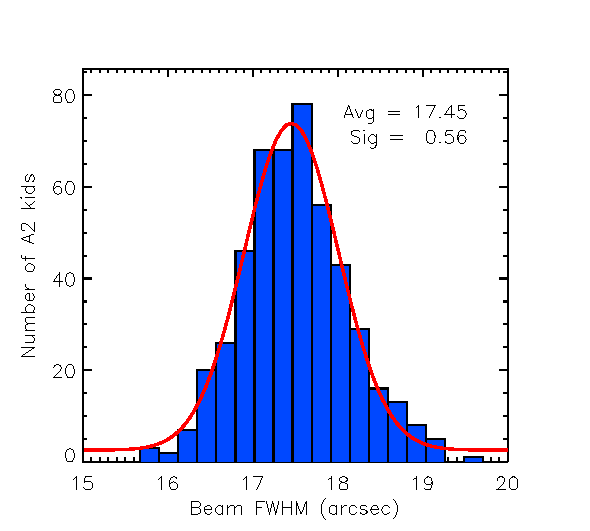
\includegraphics[clip=true,width=0.33\linewidth]{plot_histo_A2_fwhm_20170424s123.pdf}
  
\caption{From left to right, main beam FWHM distribution for arrays A1, A3, and A2 detectors. The main beam FWHM is the geometrical combination of the two-orthogonal FWHM estimates obtained from an elliptical Gaussian fit on side-lobe masked individual maps per KID (see text). The red curves show the Gaussian fit on the histogram, which provide averaged main beam FWHM of $10.9\arcsec$ at $260~\rm{GHz}$ and $17.5\arcsec$ at $150~\rm{GHz}$ in agreement with the main beam estimates from the deep beam map presented in Fig.~\ref{fig:beampattern}. The dispersion of about $0.6\arcsec$ is expected and partly due to slight change of the focus across NIKA2 FOV (of the order of -0.2~\rm{mm} at two arcmin from the FOV center).}
  \label{fig:focalplane_histo}
\end{figure*}

[LP]
Individual beams per KID across NIKA2 FOV are characterised in using
deep-integrated raster-scan observation, referred to as beam-map scan, of bright point-like
astronomical sources to project $4~\arcsec$ resolution individual maps
per KID. To isolate the main beam contribution to the total beam, the
side lodes are masked out using annulus masks centered on the peak
signal, of $50\arcsec$ external radius and of internal radius of
$9\arcsec$ at $260~\rm{GHz}$ and $14\arcsec$ at
$150~\rm{GHz}$. Elliptical 2-D Gaussian fit on the masked individual
maps provide two orthogonal-direction FWHMs, which are geometrically
combined to obtain the main beam FWHM. Figure~\ref{fig:focalplane_histo} shows the distribution of the main
beam FWHM of the array A1, A3 and A2 KID using a beam-map scan of Neptune acquired during N2R10 in average weather condition.





\subsection{Beam pattern}

\begin{figure}[h]
   \centering
    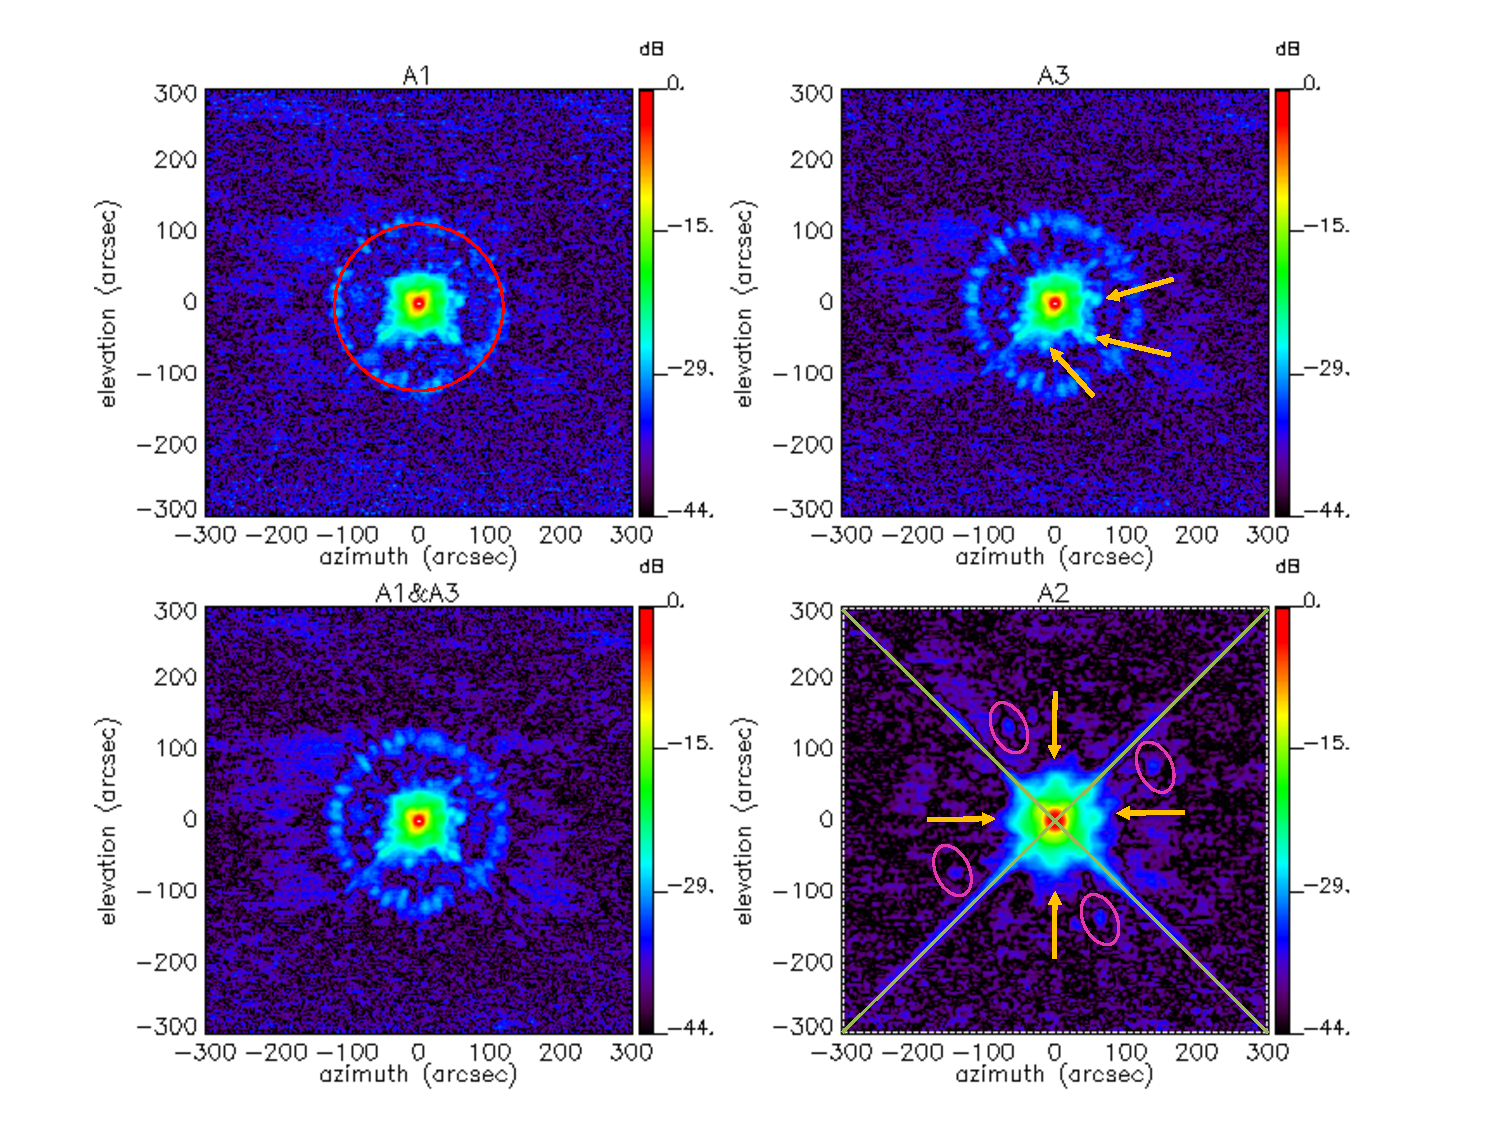
\includegraphics[width=0.9\linewidth]{Beams_features.pdf}
     
      \caption{Observed beam pattern.}
         \label{fig:beampattern}
\end{figure}

We show in Figure~\ref{}

\subsection{On-sky calibration}
\label{On-sky calibration}

\begin{figure}[h]
   \centering
    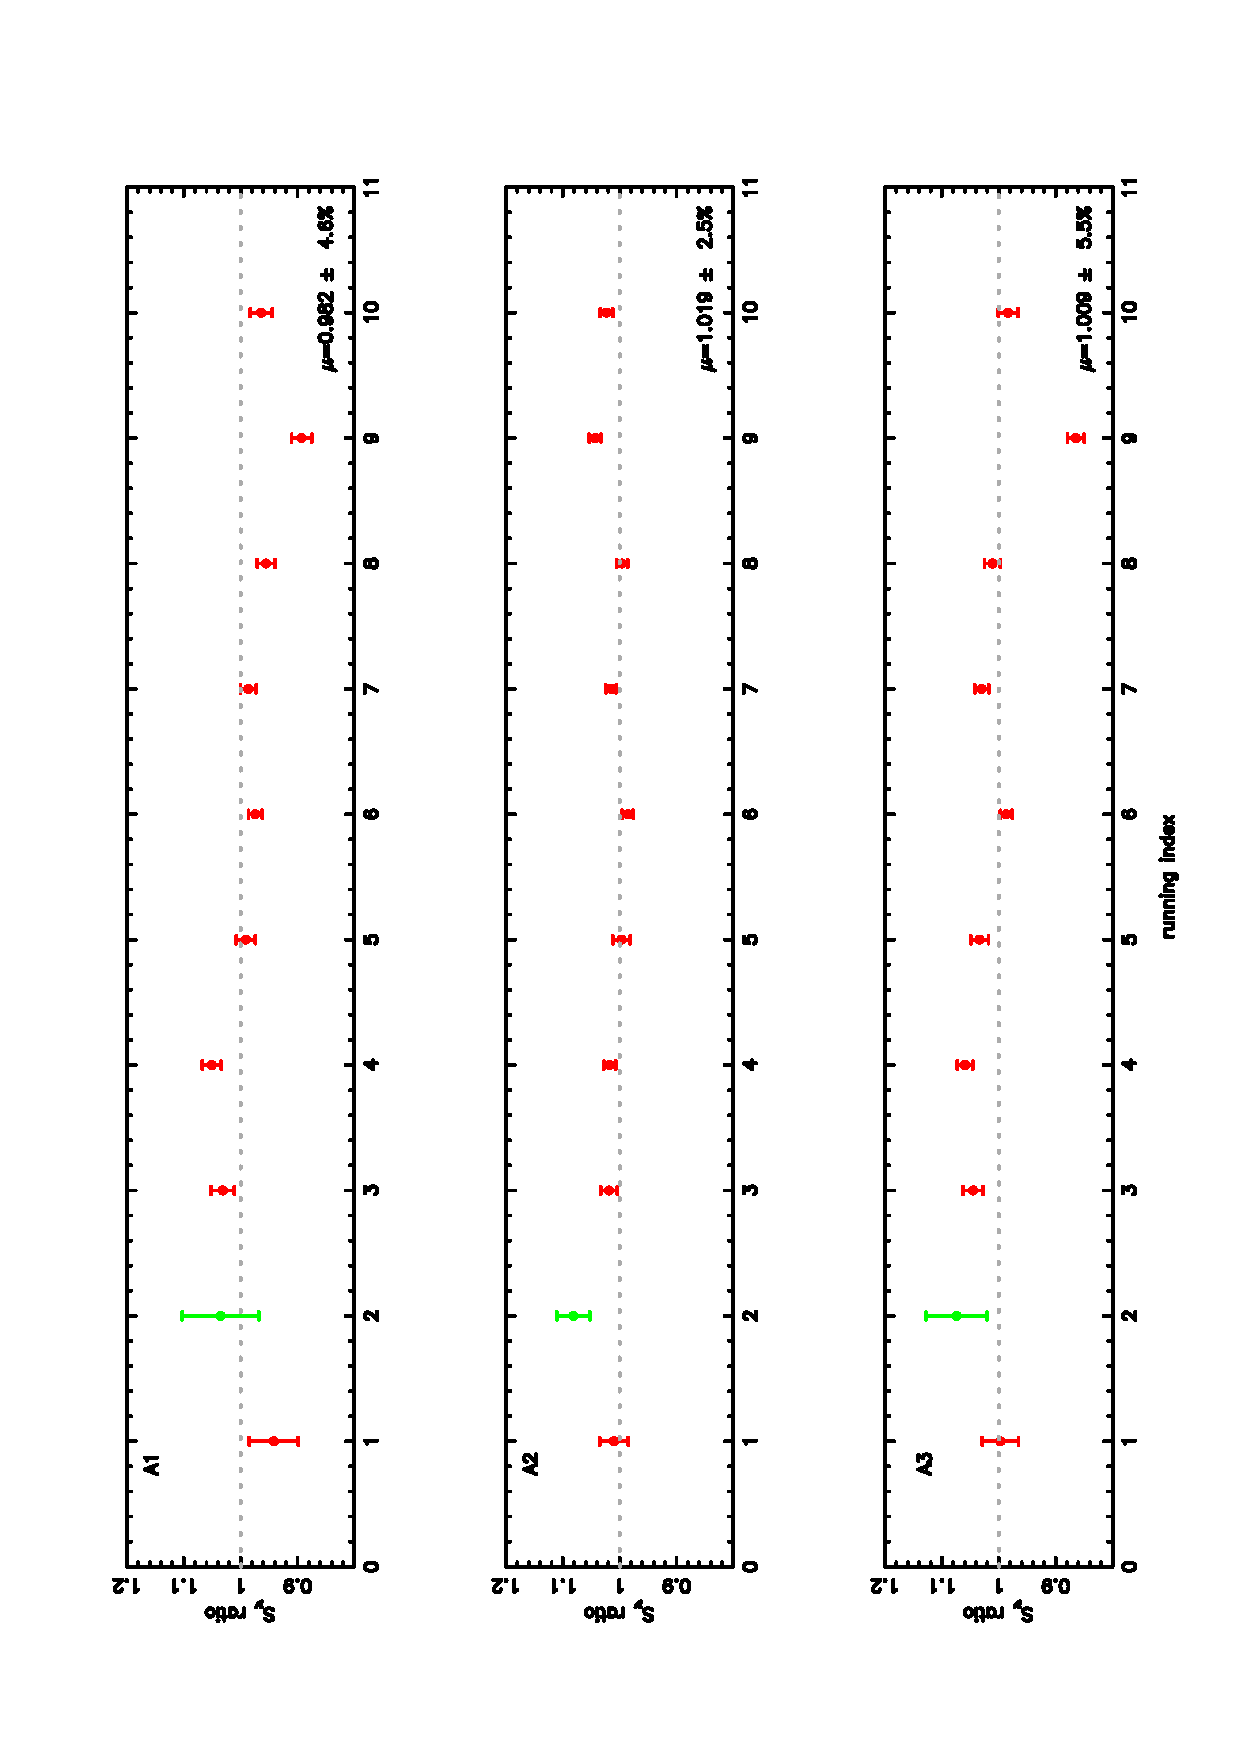
\includegraphics[angle=270,width=0.9\linewidth]{ratio_Ura_Nept.pdf}
     
      \caption{From top to bottom: primary calibrator relative flux for arrays A1, A2 and A3.}
         \label{fig:calibaccuracy}
\end{figure}

\subsection{Noise and sensitivity}
We have investigated the noise properties and sensitivity of NIKA2 in various atmospheric conditions and for various types of sources including faint and bright ones.
We find that the evolution of the noise is consistent with background noise limited detectors both at 150 and 260 GHz. Furthermore, we find that when averaging
across scans the noise evolves consistently with the square root of the time of observation.
The averaged observed sensitivity assuming 2 mm of water vapor 
and at elevation of 60 degrees are 6 and 20 mJy.s$^{1/2}$ at 150 and 260 GHz, respectively. This corresponds to average mapping speed of 180 and 2000 arcmin$^2$/hr/mJy$^2$.


\section{Compact and extended sources mapping capabilities}
During commissioning and the science verification phase we have observed several compact and extended sources in order to check the NIKA2 mapping capabilities. Here we just concentrate in few sources to illustrate the main advantages of NIKA2 with respect to previous experiments.

\subsection{Point and compact sources} 
In Figure \ref{fig_compact_sources} we present maps of MWC349 (top) and the planet Pluto(bottom) at 150 (left) and 260 (righ) GHz.
The contours represent the SNR, which reaches blablabla .
We observe MWC349 and Pluto at the center of the maps and an extra source in the edge of the map. We find for MWC349 a flux of XXX Jy.

\begin{figure*}[h]
   \centering
   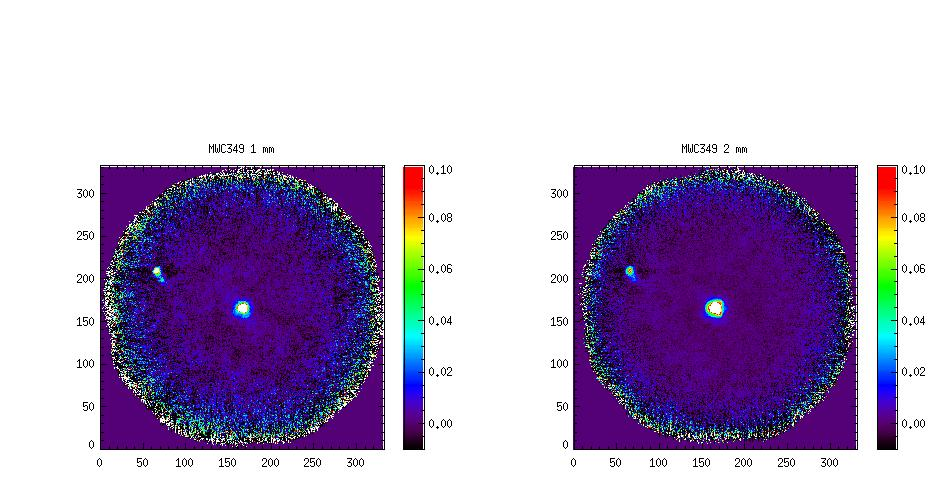
\includegraphics[width=.95\linewidth]{MWC349_v0.jpeg}
        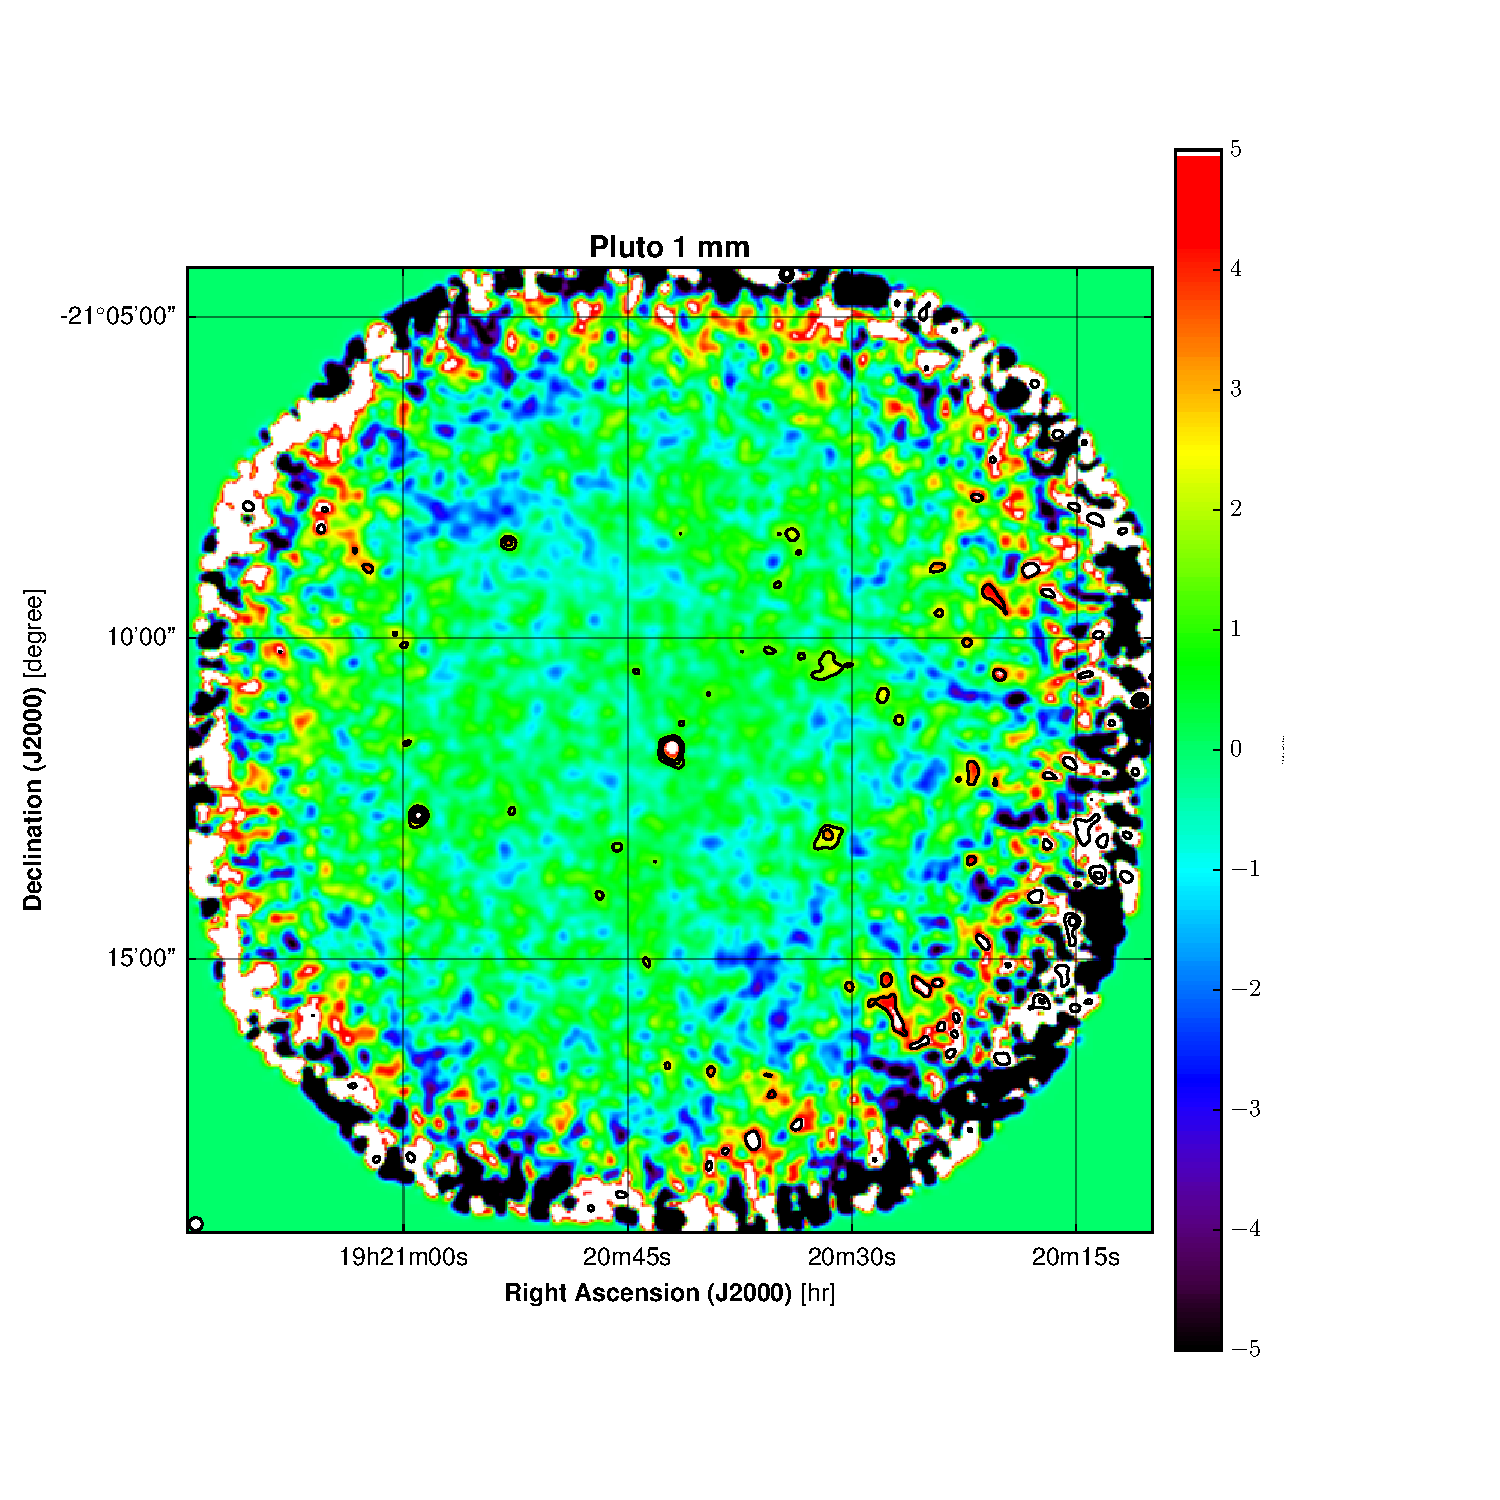
\includegraphics[width=.45\linewidth]{Pluto_1mm_map_snrcont.pdf}
    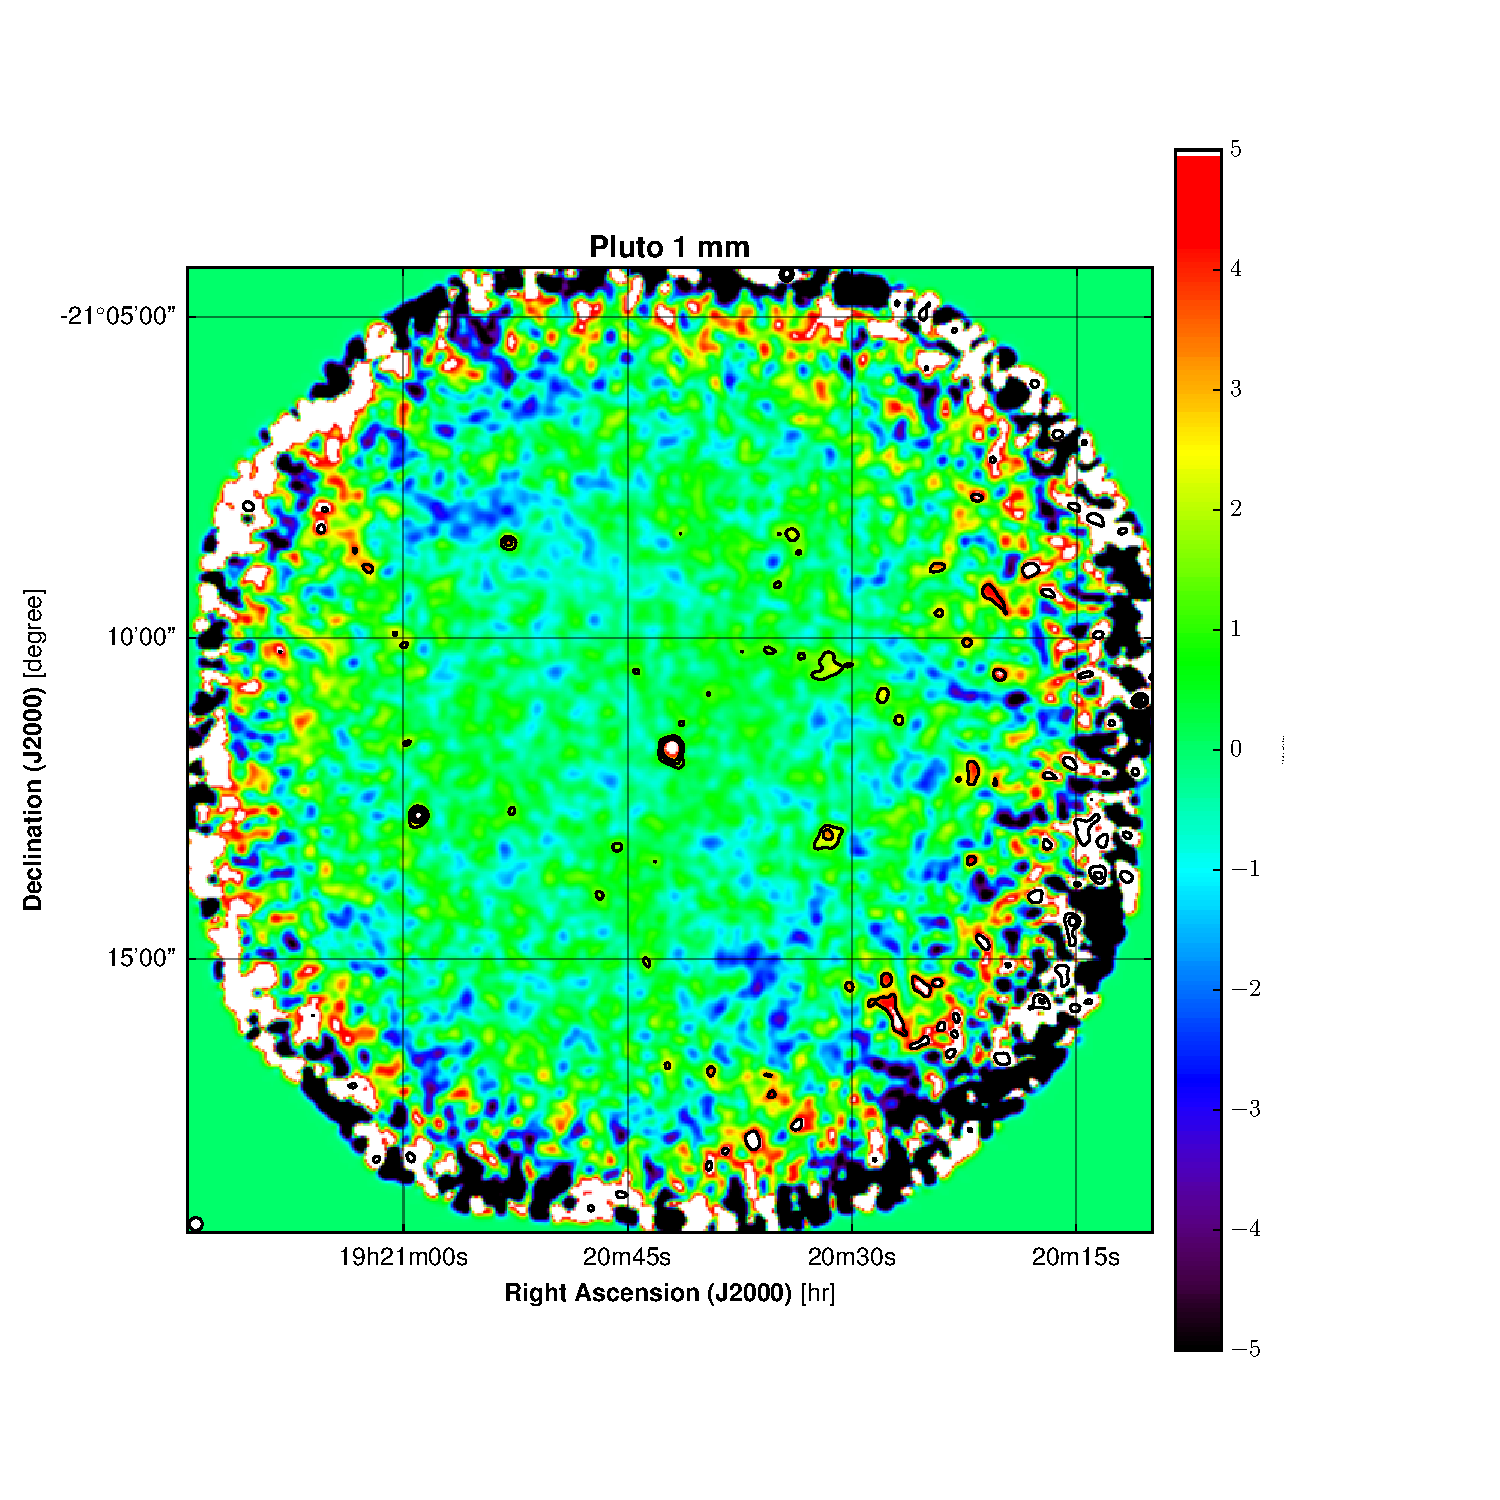
\includegraphics[width=.45\linewidth]{Pluto_1mm_map_snrcont.pdf}
      \caption{Top: Maps at 150 (left) and 260 (right) GHz of MWC349. Bottom: Maps at 150 (left) and 260 (right) GHz of the planet Pluto. {\bf change for better images}. 
         \label{fig_compact_sources}}
\end{figure*}


\subsection{Extended sources}
{\bf WE NEED TO FIND A SOURCE: why not this one (Fig.~\ref{fig:k3-50a}) (with improved display obviously
?}


\begin{figure*}[h]
   \centering
   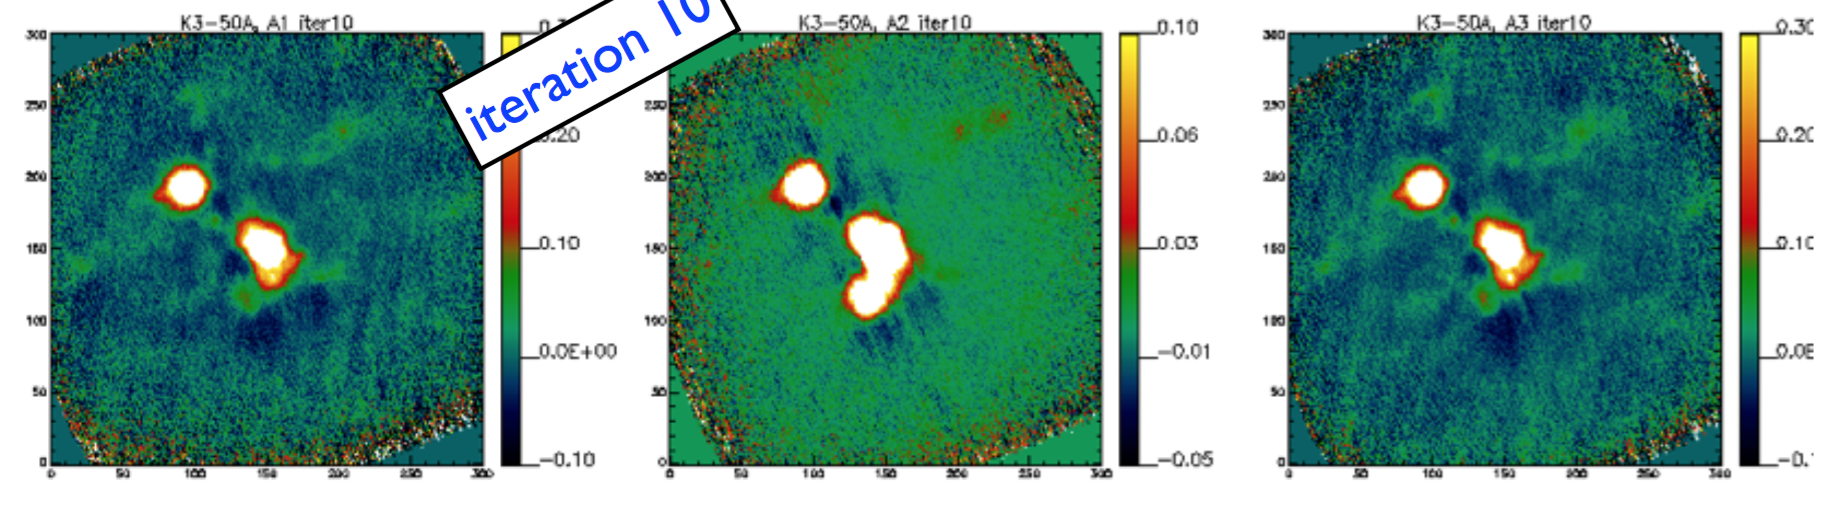
\includegraphics[width=.95\linewidth]{K3-50A.png}
   \caption{K3-50A place holder}. 
   \label{fig:k3-50a}
\end{figure*}




%WHO IN CHARGE ?? Contributions from many. Number of pages and figures you need. 1-2 possible ? 

%\subsection{Preliminary polarised maps}
%ALESSIA 

\section{Conclusions and future plans}

The NIKA2 instrument is permanently installed at the 30-meters telescope at Pico Veleta. In the present paper we have provided a general overwiew of the instrument, and given the first results obtained during the first three technical observing runs. The performance of the instrument are sufficiently good to satisfy the initial specifications already. Building on this base, NIKA2 is now allowed to enter the scientific commissioning phase. The goal is to open the instrument to the larger community during the Winter 2016/17. A more specific paper quoting final performance will be then be issued. 


\begin{acknowledgements}
{\it this is the current official NIKA2 Acknowledgements. please contact F.
Mayet if you would like to add smth.}.\\
We would like to thank the IRAM staff for their support during the campaigns. 
The NIKA dilution cryostat has been designed and built at the Institut N\'eel. 
In particular, we acknowledge the crucial contribution of the Cryogenics Group, and 
in particular Gregory Garde, Henri Rodenas, Jean Paul Leggeri, Philippe Camus. 
This work has been partially funded by the Foundation Nanoscience Grenoble, the LabEx FOCUS ANR-11-LABX-0013 and 
the ANR under the contracts "MKIDS", "NIKA" and ANR-15-CE31-0017. 
This work has benefited from the support of the European Research Council Advanced Grant ORISTARS 
under the European Union's Seventh Framework Programme (Grant Agreement no. 291294).
We acknowledge fundings from the ENIGMASS French LabEx (R. A. and F. R.), 
the CNES post-doctoral fellowship program (R. A.),  the CNES doctoral fellowship program (A. R.) and 
the FOCUS French LabEx doctoral fellowship program (A. R.).


\end{acknowledgements}

\begin{thebibliography}{16}
\expandafter\ifx\csname natexlab\endcsname\relax\def\natexlab#1{#1}\fi

\bibitem[{LTD16 2016}]{ltd16:2016}
Low Temperature Detectors LTD-16 Proceedings 2016,  Journal of Low
  Temperature Physics 184, numbers 1/2 and 3/4

\bibitem[{Monfardini {et~al.} 2011}]{Monfardini2011}
Monfardini, A., Benoit, A., Bideaud, A., {et~al.} 2011, 
The Astrophysical Journal Supplement 194, Issue 2, id. 24

\bibitem[{Catalano {et~al.} 2014}]{Catalano2014}
Catalano, A., Calvo, M., Ponthieu, N., {et~al.} 2014, 
Astronomy \& Astrophysics 569, id.A9

\bibitem[{Adam {et~al.} 2014}]{Adam2014}
Adam, R., Comis, B., Mac\'ias-P\'erez, J.-F., {et~al.} 2014, 
Astronomy \& Astrophysics 569, id.A66

\bibitem[{Day {et~al.} 2003}]{Day2003}
Day, P.~K., LeDuc, H.~G., Mazin, B.~A., Vayonakis, A., \& Zmuidzinas, J. 2003,
  Nature, 425, 817

\bibitem[{Doyle {et~al.} 2010}]{Doyle2010}
Doyle, S., Mauskopf, P., Zhang, J., {et~al.} 2008{\natexlab{a}}, in Millimeter
  and Submillimeter Detectors and Instrumentation for Astronomy IV, Proc. SPIE,
  7020, 702009

\bibitem[{Calvo {et~al.} 2010}]{Calvo2010}
Calvo, M., Giordano, C., Battiston, R., {et~al.} 2010, 
Experimental Astronomy 28, Issue 2-3, 185

\bibitem[{Roesch {et~al.} 2012}]{Roesch2012}
Roesch, M., Benoit, A., Bideaud, A., {et~al.} 2012, 
ISSTT2011 Workshop, arXiv:1212.4585

\bibitem[{Goupy {et~al.} 2016}]{Goupy2016}
Goupy, J., Adane, A., Benoit, A., {et~al.} 2016, 
Journal of Low Temperature Physics xxx, xxx, xxx

\bibitem[{Pisano {et~al.} 2016}]{Pisano2016}
Pisano, G., Xxx, X., Bbb, X., {et~al.} 2016, 
In preparation

\bibitem[{Bourrion {et~al.} 2012}]{Bourrion2012}
Bourrion, O., Vescovi, C., Bouly, J.L., {et~al.} 2012, 
Journal of Instrumentation, vol 7, P07014, arXiv:1204.1415

\bibitem[{Bourrion {et~al.} 2016}]{Bourrion2016}
Bourrion, O., Benoit, A., Bouly, J.L., {et~al.} 2016, 
Journal of Instrumentation, vol. 11, P11001, arXiv:1602.01288

\bibitem[{Swenson {et~al.} 2010}]{Swenson2010}
Swenson, L. J., Cruciani, A., Benoit, A., {et~al.} 2010, 
Applied Physics Letters 96, Issue 26, id. 263511

\bibitem[{Durand 2008}]{Durand2008}
Durand, T., 2008, 
PhD Thesis, Universit\' e de Grenoble

\bibitem[{Calvo {et~al.} 2013}]{Calvo2013}
Calvo, M., Roesch, M., D\'esert, F.-X., {et~al.} 2013, 
Astronomy \& Astrophysics 551, id.L12

\bibitem[{Pardo {et~al.} 2002}]{2001IEEE....49.1683C}
Pardo J.~R., Cernicharo J., Serabyn E., 2002, 
IEEE, 49, 1683 - 1694


\end{thebibliography}

%\bibliographystyle{aa}
%\bibliography{biblio_NIKA2} 

\end{document}



%%%%%%%%%%%%%%%%%%%%%%%%%%%%%%%%%%%%%%%%%%%%%%%%%%%%%%%%%%%%%%
Examples for figures using graphicx
A guide "Using Imported Graphics in LaTeX2e"  (Keith Reckdahl)
is available on a lot of LaTeX public servers or ctan mirrors.
The file is : epslatex.pdf
%%%%%%%%%%%%%%%%%%%%%%%%%%%%%%%%%%%%%%%%%%%%%%%%%%%%%%%%%%%%%%

%_____________________________________________________________
%                 A figure as large as the width of the column
%-------------------------------------------------------------
   \begin{figure}
   \centering
   \includegraphics[width=\textwidth]{empty.eps}
      \caption{Vibrational stability equation of state
               $S_{\mathrm{vib}}(\lg e, \lg \rho)$.
               $>0$ means vibrational stability.
              }
         \label{FigVibStab}
   \end{figure}
%
%_____________________________________________________________
%                                    One column rotated figure
%-------------------------------------------------------------
   \begin{figure}
   \centering
   \includegraphics[angle=-90,width=3cm]{empty.eps}
      \caption{Vibrational stability equation of state
               $S_{\mathrm{vib}}(\lg e, \lg \rho)$.
               $>0$ means vibrational stability.
              }
         \label{FigVibStab}
   \end{figure}
%
%_____________________________________________________________
%                        Figure with caption on the right side
%-------------------------------------------------------------
   \begin{figure}
   \centering
   \includegraphics[width=3cm]{empty.eps}
      \caption{Vibrational stability equation of state
               $S_{\mathrm{vib}}(\lg e, \lg \rho)$.
               $>0$ means vibrational stability.
              }
         \label{FigVibStab}
   \end{figure}
%
%_____________________________________________________________
%
%_____________________________________________________________
%                                Figure with a new BoundingBox
%-------------------------------------------------------------
   \begin{figure}
   \centering
   \includegraphics[bb=10 20 100 300,width=3cm,clip]{empty.eps}
      \caption{Vibrational stability equation of state
               $S_{\mathrm{vib}}(\lg e, \lg \rho)$.
               $>0$ means vibrational stability.
              }
         \label{FigVibStab}
   \end{figure}
%
%_____________________________________________________________
%
%_____________________________________________________________
%                                      The "resizebox" command
%-------------------------------------------------------------
   \begin{figure}
   \resizebox{\textwidth}{!}
            {\includegraphics[bb=10 20 100 300,clip]{empty.eps}
      \caption{Vibrational stability equation of state
               $S_{\mathrm{vib}}(\lg e, \lg \rho)$.
               $>0$ means vibrational stability.
              }
         \label{FigVibStab}
   \end{figure}
%
%______________________________________________________________
%
%_____________________________________________________________
%                                             Simple A&A Table
%_____________________________________________________________
%
\begin{table}
\caption{Nonlinear Model Results}             % title of Table
\label{table:1}      % is used to refer this table in the text
\centering                          % used for centering table
\begin{tabular}{c c c c}        % centered columns (4 columns)
\hline\hline                 % inserts double horizontal lines
HJD & $E$ & Method\#2 & Method\#3 \\    % table heading
\hline                        % inserts single horizontal line
   1 & 50 & $-837$ & 970 \\      % inserting body of the table
   2 & 47 & 877    & 230 \\
   3 & 31 & 25     & 415 \\
   4 & 35 & 144    & 2356 \\
   5 & 45 & 300    & 556 \\
\hline                                   %inserts single line
\end{tabular}
\end{table}
%
%_____________________________________________________________
%                                             Two column Table
%_____________________________________________________________
%
\begin{table*}
\caption{Nonlinear Model Results}
\label{table:1}
\centering
\begin{tabular}{c c c c l l l }     % 7 columns
\hline\hline
                      % To combine 4 columns into a single one
HJD & $E$ & Method\#2 & \multicolumn{4}{c}{Method\#3}\\
\hline
   1 & 50 & $-837$ & 970 & 65 & 67 & 78\\
   2 & 47 & 877    & 230 & 567& 55 & 78\\
   3 & 31 & 25     & 415 & 567& 55 & 78\\
   4 & 35 & 144    & 2356& 567& 55 & 78 \\
   5 & 45 & 300    & 556 & 567& 55 & 78\\
\hline
\end{tabular}
\end{table*}
%
%_____________________________________________________________
%                                          Table with foonotes
%-------------------------------------------------------------
%
\begin{table}
\begin{minipage}[t]{\columnwidth}
\caption{LHNW source catalogue.}
\label{catalog}
\centering
\renewcommand{\footnoterule}{}  % to avoid a line before footnotes
\begin{tabular}{lccccc}
\hline \hline
ID& RA     &  Dec    & {\it S/N} & Flux  \\
~ &(J2000) & (J2000) &~    & [{\rm mJy}] \\
\hline
   LHJ10  &10:32:02.4  &     +58:80:09  &   8  &    97 $\pm$  15\\
   LHJ10  &10:33:08.8  &     +58:80:30  &   5  &    80 $\pm$  16\\
   LHJ10  &10:34:45.1  &     +57:47:33\footnote{Text of the footnote}
                                               &   5  &    48 $\pm$  10\\
   LHJ10  &10:32:49.7  &     +57:37:19  &   5  &    56 $\pm$  11\\
   LHJ10  &10:33:52.1  &     +58:40:30\footnote{Text of the footnote}
                                               &   4  &    55 $\pm$  14\\
   LHJ10  &10:33:04.3  &     +57:36:37  &   4  &    55 $\pm$  14\\
   LHJ10  &10:35:50.4  &     +57:30:05  &   4  &    49 $\pm$  11\\
\hline
\end{tabular}
\end{minipage}
\end{table}
%
%_____________________________________________________________
%                                 A rotated Table in landscape
%  In the preamble, use:   \usepackage{lscape}
%-------------------------------------------------------------
\begin{landscape}
\begin{table*}
\caption{Summary for ISOCAM sources with mid-IR excess
(YSO candidates).}\label{YSOtable}
\centering
\begin{tabular}{crrlcl}
\hline\hline
ISO-L1551 & $F_{6.7}$~[mJy] & $\alpha_{6.7-14.3}$
& YSO type$^{d}$ & Status & Comments\\
\hline
  \multicolumn{6}{c}{\it New YSO candidates}\\ % To combine 6 columns into a single one
\hline
  1 & 1.56 $\pm$ 0.47 & --    & Class II$^{c}$ & New & Mid\\
  2 & 0.79:           & 0.97: & Class II ?     & New & \\
  3 & 4.95 $\pm$ 0.68 & 3.18  & Class II / III & New & \\
  5 & 1.44 $\pm$ 0.33 & 1.88  & Class II       & New & \\
\hline
  \multicolumn{6}{c}{\it Previously known YSOs} \\
\hline
  61 & 0.89 $\pm$ 0.58 & 1.77 & Class I & \object{HH 30} & Circumstellar disk\\
  96 & 38.34 $\pm$ 0.71 & 37.5& Class II& MHO 5          & Spectral type\\
\hline
\end{tabular}
\end{table*}
\end{landscape}
%
%_____________________________________________________________
%                              Table longer than a single page
%  In the preamble, use:              \usepackage{longtable}
%-------------------------------------------------------------
%          All long tables have to be placed at the end, after
%                                        \end{thebibliography}
%
% In the text, at the place where the large table should appear
% add the command:
\addtocounter{table}{1}
% Tables counters will be well numbered.
%
\end{thebibliography}
% If table 2
\longtab{2}{
\begin{longtable}{lllrrr}
\caption{\label{kstars} Sample stars with absolute magnitude}\\
\hline\hline
Catalogue& $M_{V}$ & Spectral & Distance & Mode & Count Rate \\
\hline
\endfirsthead
\caption{continued.}\\
\hline\hline
Catalogue& $M_{V}$ & Spectral & Distance & Mode & Count Rate \\
\hline
\endhead
\hline
\endfoot
%%
Gl 33    & 6.37 & K2 V & 7.46 & S & 0.043170\\
Gl 66AB  & 6.26 & K2 V & 8.15 & S & 0.260478\\
Gl 68    & 5.87 & K1 V & 7.47 & P & 0.026610\\
         &      &      &      & H & 0.008686\\
Gl 86
\footnote{Source not included in the HRI catalog. See Sect.~5.4.2 for details.}
         & 5.92 & K0 V & 10.91& S & 0.058230\\
\end{longtable}
}% End \longtab
%
%_____________________________________________________________
%                              Table longer than a single page
%                                             and in landscape
%  In the preamble, use:       \usepackage{longtable,lscape}
%-------------------------------------------------------------
%          All long tables have to be placed at the end, after
%                                        \end{thebibliography}
%
% In the text, at the place where the large table should appear
% add the command:
\addtocounter{table}{1}
% Tables counters will be well numbered.
%
\end{thebibliography}
% If table 2
\longtabL{2}{
\begin{landscape}
\begin{longtable}{lllrrr}
\caption{\label{kstars} Sample stars with absolute magnitude}\\
\hline\hline
Catalogue& $M_{V}$ & Spectral & Distance & Mode & Count Rate \\
\hline
\endfirsthead
\caption{continued.}\\
\hline\hline
Catalogue& $M_{V}$ & Spectral & Distance & Mode & Count Rate \\
\hline
\endhead
\hline
\endfoot
%%
Gl 33    & 6.37 & K2 V & 7.46 & S & 0.043170\\
Gl 66AB  & 6.26 & K2 V & 8.15 & S & 0.260478\\
Gl 68    & 5.87 & K1 V & 7.47 & P & 0.026610\\
         &      &      &      & H & 0.008686\\
Gl 86
\footnote{Source not included in the HRI catalog. See Sect.~5.4.2 for details.}
         & 5.92 & K0 V & 10.91& S & 0.058230\\
\end{longtable}
\end{landscape}
}% End \longtabL
%
% Online Material
%_____________________________________________________________
%        Online appendices have to be placed at the end, after
%                                        \end{thebibliography}
%-------------------------------------------------------------
\end{thebibliography}

\Online

\begin{appendix} %First online appendix
\section{Background galaxy number counts and shear noise-levels}
Because the optical images used in this analysis...

\begin{figure*}
\centering
\includegraphics[width=16.4cm,clip]{1787f24.ps}
\caption{Plotted above...}
\label{appfig}
\end{figure*}

Because the optical images...
\end{appendix}

\begin{appendix} %Second online appendix
These studies, however, have faced...
\end{appendix}

\end{document}
%
%_____________________________________________________________
%        Some tables or figures are in the printed version and
%                      some are only in the electronic version
%-------------------------------------------------------------
%
% Leave all the tables or figures in the text, at their right place
% and use the commands \onlfig{}{} and \onltab{}{}. These elements
% will be automatically placed at the end, in the section
% Online material.

\documentclass{aa}
...
\begin{document}
text of the paper...
\begin{figure*}%f1
\includegraphics[width=10.9cm]{1787f01.eps}
\caption{Shown in greyscale is a...}
\label{cl12301}}
\end{figure*}
...
from the intrinsic ellipticity distribution.
% Figure 2 available electronically only
\onlfig{2}{
\begin{figure*}%f2
\includegraphics[width=11.6cm]{1787f02.eps}
\caption {Shown in greyscale...}
\label{cl1018}
\end{figure*}
}

% Figure 3 available electronically only
\onlfig{3}{
\begin{figure*}%f3
\includegraphics[width=11.2cm]{1787f03.eps}
\caption{Shown in panels...}
\label{cl1059}
\end{figure*}
}

\begin{figure*}%f4
\includegraphics[width=10.9cm]{1787f04.eps}
\caption{Shown in greyscale is...}
\label{cl1232}}
\end{figure*}

\begin{table}%t1
\caption{Complexes characterisation.}\label{starbursts}
\centering
\begin{tabular}{lccc}
\hline \hline
Complex & $F_{60}$ & 8.6 &  No. of  \\
...
\hline
\end{tabular}
\end{table}
The second method produces...

% Figure 5 available electronically only
\onlfig{5}{
\begin{figure*}%f5
\includegraphics[width=11.2cm]{1787f05.eps}
\caption{Shown in panels...}
\label{cl1238}}
\end{figure*}
}

As can be seen, in general the deeper...
% Table 2 available electronically only
\onltab{2}{
\begin{table*}%t2
\caption{List of the LMC stellar complexes...}\label{Properties}
\centering
\begin{tabular}{lccccccccc}
\hline  \hline
Stellar & RA & Dec & ...
...
\hline
\end{tabular}
\end{table*}
}

% Table 3 available electronically only
\onltab{3}{
\begin{table*}%t3
\caption{List of the derived...}\label{IrasFluxes}
\centering
\begin{tabular}{lcccccccccc}
\hline \hline
Stellar & $f12$ & $L12$ &...
...
\hline
\end{tabular}
\end{table*}
}
%
%-------------------------------------------------------------
%     For the online material, table longer than a single page
%                 In the preamble, use: \usepackage{longtable}
%       or for landscape option: \usepackage{longtable,lscape}
%-------------------------------------------------------------
\documentclass{aa}
\usepackage[varg]{txfonts}
\usepackage{graphicx}
\usepackage{longtable}

\begin{document}
text of the paper
% Table will be print automatically at the end, in the section Online material.
\onllongtab{3}{
\begin{longtable}{lrcrrrrrrrrl}
\caption{Line data and abundances ...}\\
\hline
\hline
Def & mol & Ion & $\lambda$ & $\chi$ & $\log gf$ & N & e &  rad & $\delta$ & $\delta$
red & References \\
\hline
\endfirsthead
\caption{Continued.} \\
\hline
Def & mol & Ion & $\lambda$ & $\chi$ & $\log gf$ & B & C &  rad & $\delta$ & $\delta$
red & References \\
\hline
\endhead
\hline
\endfoot
\hline
\endlastfoot
A & CH & 1 &3638 & 0.002 & $-$2.551 &  &  &  & $-$150 & 150 &  Jorgensen et al. (1996) \\
\end{longtable}
}% End onllongtab

% Or for landscape, large table:

\onllongtabL{3}{
\begin{landscape}
\begin{longtable}{lrcrrrrrrrrl}
...
\end{longtable}
\end{landscape}
}% End onllongtabL
